% =============================================================================
% glyphs
% =============================================================================

\chapter{Entity Relationship glyphs}
\label{chp:glyph}

This chapter provides a catalog of the graphical symbols available for representing entities in \ERms.  There are different classes of glyphs corresponding to different classes of entity nodes, statements and influences.

In \chap{grammar} beginning on page~\pageref{chp:grammar}, we describe the rules for combining these glyphs into legal SBGN \ERs, and in \chap{layout} beginning on page~\pageref{chp:layout}, we describe requirements and guidelines for the way that maps are visually organized.

\section{Overview}
 
% =============================================================================
% overview
% =============================================================================

To set the stage for what follows in this chapter, we first give a brief overview of some of the concepts in the \ER notation with the help of an example shown in \fig{eg1}. This example will be re-used throughout the description of the graphical symbols (glyphs) used by \SBGNERLone (with a few additions when the concepts are missing in the example) 

\begin{figure}[H]
  \centering
  \vspace*{-0.75em}
  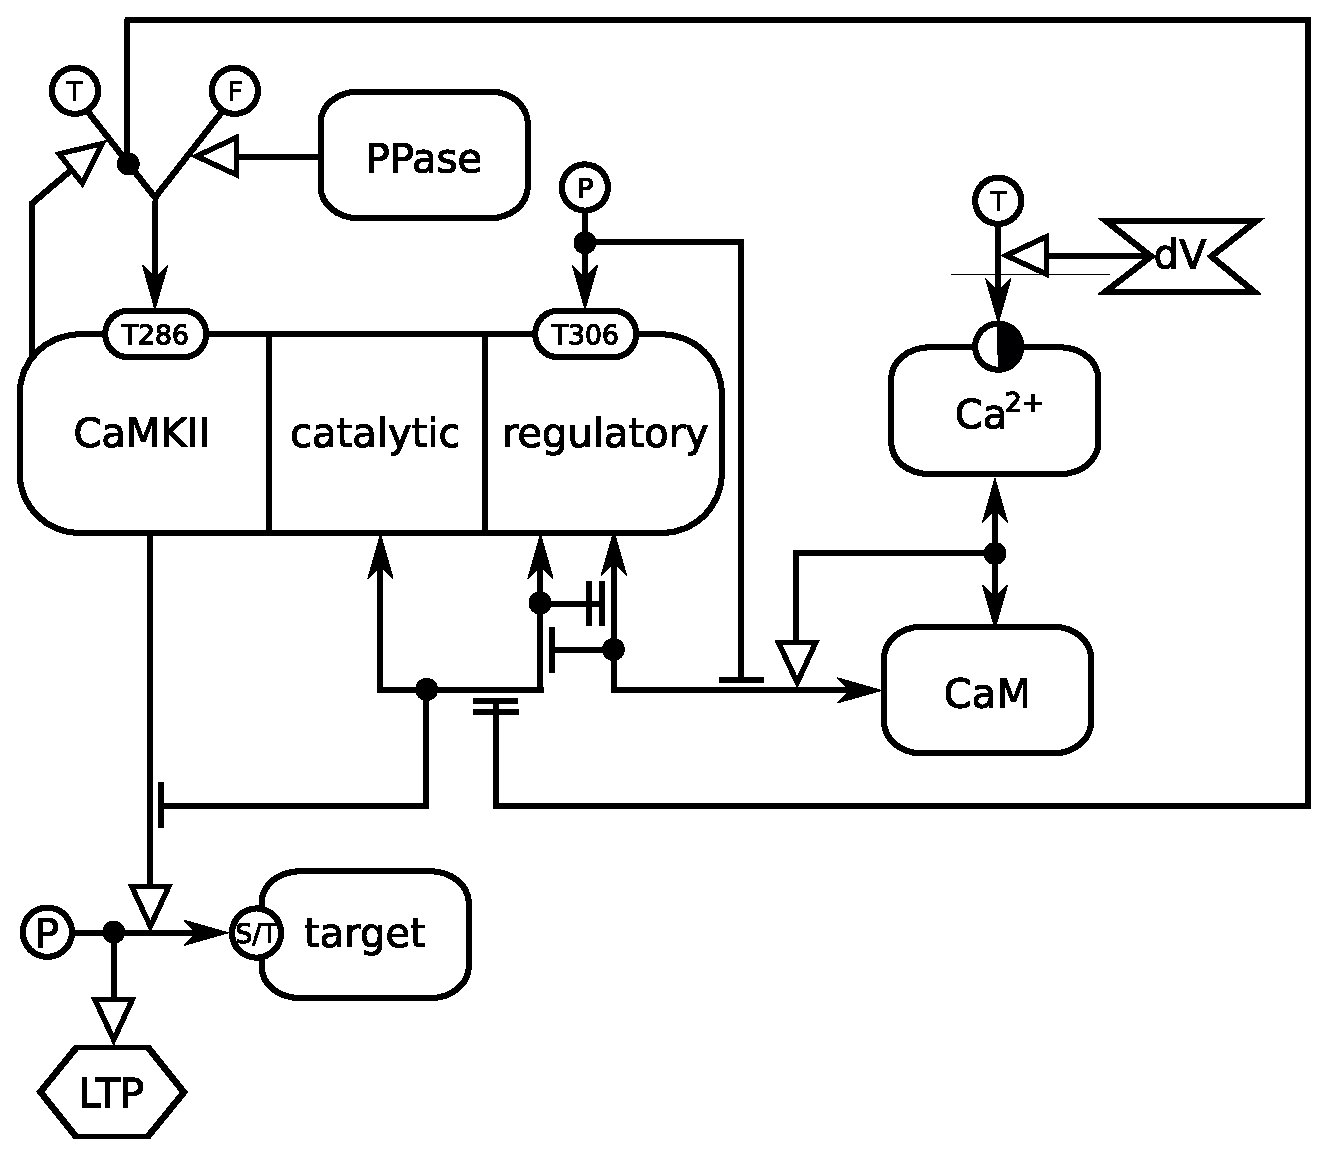
\includegraphics[scale=0.6]{examples/CaMKII-intro}
   \caption{This example of a \ER diagram depicts the effect of a depolarisation (dV) on the intracellular calcium, that binds to Calmodulin (CaM), that itself binds to the calcium/calmoduline kinase II (CaMKII). The binding of calmodulin inhibits the interaction between the catalytic and regulatory domains, thus relieving the inhibition on the kinase activity. The phosphorylation of the targets finally leads to the Long Term Potentiation (LTP) of the synapses. In addition, the diagram shows the effect of phosphorylation on threonine 286, that makes the enzyme constitutively active, and on threonine 306, that renders the kinase insensitive to calmodulin.}
  \label{fig:eg1}
\end{figure}
 
The essence of the \ER diagram is to depict the influences of entities upon the behaviour of others. The entities (in fact all interactors) are things that exist, either on their own or when statements become true. For instance, an entity can exist, different entities can interact, or a value can be assigned to an entity's property. The influences can therefore be understood as logical consequences of this existence. Contrary to the Process Diagram notation, where the different processes affect each other, the relationships are independent. On can imagine that each of the relationships represent a specific conclusion of a scientific experience or article. Their addition on a map represent the extend a the knowledge we have of the effects of the entities represented upon each other. The independence of relationships is the key to avoid the combinatorial explosion inherent to Process Diagrams.

\tab{component-summary} summarizes the different SBGN abstractions described in this chapter.
 
\newcolumntype{P}[1]{>{\raggedright\hspace{0pt}\arraybackslash}p{#1}}
 
 \begin{table}[h]
   \centering
   \small
   \begin{tabular}{@{}lP{2.4in}P{2.4in}@{}}
     \toprule
     \textbf{Component} & \textbf{Role} & \textbf{Examples}\\
     \midrule
     Interactor node
     & Something that exists
     & An entity, the result of an interaction \\[0.5em]
 
     Statement	
     & Something that can be true or false
     & An interaction between entities, the assignment of a value to a variable \\[0.5em]
 
     Influence
     & The effect of something true on the realisation of a statement or another influence.
     & A stimulation, an absolute inhibition \\
     \bottomrule
   \end{tabular}
   \caption{Summary of \ER components and their roles.}
   \label{tab:component-summary}
 \end{table}


 
\section{Controlled vocabularies used in \SBGNERLone}\label{sec:CVs}

%%%%%%%%%%%%%%%%%%%%%%%%%%%%%%%%%%%%%%%%%%%%%%%%%%%%%%%%%%%%%%%%%%%%%%
%%%%                   Controlled vocabularies
%%%%%%%%%%%%%%%%%%%%%%%%%%%%%%%%%%%%%%%%%%%%%%%%%%%%%%%%%%%%%%%%%%%%%%

\section{Controlled vocabularies used in \SBGNERLone}\label{sec:CVs}

Some glyphs in SBGN \ERs can contain particular kinds of textual annotations conveying information relevant to the purpose of the glyph.  These annotations are carried by \glyph{units of information} (\sect{unitInformation}) or \glyph{state variable values} (\sect{stateVariable}).

The text that appears as the unit of information decorating an entity must be prefixed with a controlled vocabulary term indicating the type of information being expressed.  The prefixes are mandatory.  Without the use of controlled vocabulary prefixes, it would be necessary to have different glyphs to indicate different classes of information; this would lead to an explosion in the number of symbols needed.

In the rest of this section, we describe the controlled vocabularies (CVs) used in \SBGNERLone.  In each case, some CV terms are predefined by SBGN, but unless otherwise noted, \emph{they are not the only terms permitted}.  Authors may use other CV values not listed here, but in such cases, they should explain the terms' meanings in a figure legend or other text accompanying the map.

\subsection{Entity material types}
\label{sec:material-types-cv}

The material type of an \glyph{Entity} indicates its chemical structure.  A list of common material types is shown in \fig{material-types-cv}, but others are possible.  The values are to be taken from the \sbo (\sbourl), specifically from the branch having identifier \sboid{SBO:0000240} (\emph{material entity}).  The labels are defined by \SBGNERLone.

\begin{figure}[h]
  \centering
  \begin{tabular}{l>{\ttfamily}ll}
    \toprule
    \textbf{Name}              & \textbf{\rmfamily Label} & \textbf{SBO term} \\
    \midrule
    Non-macromolecular ion     & mt:ion  & SBO:0000327\\
    Non-macromolecular radical & mt:rad  & SBO:0000328\\
    Ribonucleic acid           & mt:rna  & SBO:0000250\\
    Deoxribonucleic acid       & mt:dna  & SBO:0000251\\
    Protein                    & mt:prot & SBO:0000297\\
    Polysaccharide             & mt:psac & SBO:0000249\\
    \bottomrule
  \end{tabular}
  \caption{A sample of values from the \emph{material types} controlled
    vocabulary (\sect{material-types-cv}).}
  \label{fig:material-types-cv}
\end{figure}

The material types are in contrast to the \emph{conceptual types} (see below).  The distinction is that material types are about physical composition, while conceptual types are about functions.  For example, a strand of RNA is a physical artifact, but its use as messenger RNA is a function.

\subsection{Entity conceptual types}
\label{sec:conceptual-types-cv}

An \glyph{entity}'s \emph{conceptual type} indicates its function within the context of a given \ERm.  A list of common conceptual types is shown in \fig{conceptual-types-cv}, but others are possible.  The values are to be taken from the \sbo (\sbourl), specifically from the branch having identifier \sboid{SBO:0000241} (\emph{functional entity}).  The labels are defined by \SBGNERLone.

\begin{figure}[h]
  \centering
  \begin{tabular}{l>{\ttfamily}ll}
    \toprule
    \textbf{Name}              & \textbf{\rmfamily Label} & \textbf{SBO term} \\
    \midrule
    Gene                      & ct:gene   & SBO:0000243\\
    Transcription start site  & ct:tss    & SBO:0000329\\
    Gene coding region        & ct:coding & SBO:0000335\\
    Gene regulatory region    & ct:grr    & SBO:0000369\\
    Messenger RNA             & ct:mRNA   & SBO:0000278\\
    Functional domain         & ct:domain & SBO:0000493\\
    Binding site              & ct:bind   & SBO:0000494\\
    Catalytic site            & ct:cat    & SBO:0000495\\
    Transmembrane domain      & ct:tm     & SBO:0000496\\
    \bottomrule
  \end{tabular}
  \caption{A sample of values from the \emph{conceptual types} vocabulary
    (\sect{conceptual-types-cv}).}
  \label{fig:conceptual-types-cv}
\end{figure}

\subsection{Macromolecule covalent modifications}
\label{sec:covalent-mod-cv}

A common reason for the introduction of state variables on an entity is to allow access to the configuration of possible covalent modification sites on that entity.  For instance, a macromolecule may have one or more sites where a phosphate group may be attached; this change in the site's configuration (\ie being either phosphorylated or not) may factor into whether, and how, the entity can participate in different processes.  Being able to describe such modifications in a consistent fashion is the motivation for the existence of SBGN's covalent modifications controlled vocabulary.  

\fig{covalent-mod-cv} lists a number of common types of covalent modifications.  The most common values are defined by the \sbo in the branch having identifier \sboid{SBO:0000210} (\emph{addition} under \emph{events}$\rightarrow$\emph{reaction}$\rightarrow$\emph{biochemical reaction}$\rightarrow$\emph{conversion}$\rightarrow$\emph{addition}).  The labels shown in \fig{covalent-mod-cv} are defined by \SBGNERLone; for all other kinds of modifications not listed here, the author of an \ERm must create a new label (and should also describe the meaning of the label in a legend or text accompanying the map).

\begin{figure}[h]
  \centering
  \begin{tabular}{l>{\ttfamily}ll}
    \toprule
    \textbf{Name}   & \textbf{\rmfamily Label} & \textbf{SBO term} \\
    \midrule
    Acetylation     & Ac    & SBO:0000215\\
    Glycosylation   & G     & SBO:0000217\\
    Hydroxylation   & OH    & SBO:0000233\\
    Methylation     & Me    & SBO:0000214\\
    Myristoylation  & My    & SBO:0000219\\
    Palmytoylation  & Pa    & SBO:0000218\\
    Phosphorylation & P     & SBO:0000216\\
    Prenylation     & Pr    & SBO:0000221\\
    Protonation     & H     & SBO:0000212\\
    Sulfation       & S     & SBO:0000220\\
    Ubiquitination  & Ub    & SBO:0000224\\
    \bottomrule
  \end{tabular}
  \caption{A sample of values from the \emph{covalent modifications} vocabulary
    (\sect{covalent-mod-cv}).}
  \label{fig:covalent-mod-cv}
\end{figure}

\subsection{Miscellaneous terms}
\label{sec:miscellaneous-cv}

\SBGNERLone requires several reserved characters. A special unit of information usable on interactions describe the number of identical interactors involved. Note that the value is a unitary number, and not (for example) a range.  There is no provision in \SBGNPDLone for specifying a range in this context because it leads to problems of entity identifiability. Other reserved characters are used in state variable assignments to represent truth or falsehood. Two reserved words are used in units of information carried by relationships: cis and trans. 

\begin{table}[h]
  \centering
  \begin{tabular}{l>{\ttfamily}l>{\ttfamily}l}
    \toprule
    \textbf{Name}   & \textbf{\rmfamily Label} & \textbf{\rmfamily SBO term} \\
    \midrule
    cardinality    & \#  & SBO:0000364\\
    true           & T     & SBO:0000416\\
    false          & F     & SBO:0000417\\
    cis            & cis   & SBO:0000414\\
    trans          & trans & SBO:0000415\\
    \bottomrule
  \end{tabular}
  \caption{Miscellaneous controlled terms. For the cardinality, \texttt{\#} stands for a number, for example, ``\texttt{5}''.}
  \label{tab:cardinality-cv}
\end{table}

%\normalcolor

 
 %%%%%%%%%%%%%%%%%%%%%%%%%%%%%%%%%%%%%%%%%%%%%%%%%%%%%%%%%%%%%%%%%%%%%%
 %%%%%%%%%%%%%%%%%%%%%%%%%%%%%%%%%%%%%%%%%%%%%%%%%%%%%%%%%%%%%%%%%%%%%%
 %%%%                   Interactor nodes
 %%%%%%%%%%%%%%%%%%%%%%%%%%%%%%%%%%%%%%%%%%%%%%%%%%%%%%%%%%%%%%%%%%%%%%
 %%%%%%%%%%%%%%%%%%%%%%%%%%%%%%%%%%%%%%%%%%%%%%%%%%%%%%%%%%%%%%%%%%%%%%
 
\section{Entity nodes}\label{sec:ENs}

\glyph{Entity nodes} (ENs) represent element of truth, things that exist. 
%In ontology parlance, they would be ``continuants''. 
Entity nodes are the source of influences. \SBGNERLone{} provides three different types of \glyph{entity nodes}, the \glyph{interactors}, the \glyph{logical operators} and the \glyph{perturbing agent}. 

\subsection{Interactors}\label{sec:interactors}

Interactors are entity nodes that are able to participate in an interaction (\sect{interaction}). \SBGNERLone{} provides two interactors, the \glyph{entity} and the \glyph{outcome} of a statement.

%%%%%%%%%%%%%%%%%%%%%%%%%%%%%%%%%%%%%%%%%%%%%%%%%%%%%%%%%%%%%%%%%%%%%%
%%                     Entity
%%%%%%%%%%%%%%%%%%%%%%%%%%%%%%%%%%%%%%%%%%%%%%%%%%%%%%%%%%%%%%%%%%%%%%
\color{green}

\subsection{Glyph: \glyph{Entity}}
\label{sec:entity}

\SBGNERLone defines only one glyph for all entities, whether physical entity, such as protein, a nucleic acid, metabolite or functional entity such as a gene. Indeed the exact nature of entities does not impact the rules of interactions within a diagram. The nature of a particular entity may then be clarified using its label and decorations, as will become clear below. 

\begin{glyphDescription}

\glyphSboTerm SBO:0000245 ! entity 

\glyphContainer An entity is represented by a rectangular container with rounded corners, as illustrated in \fig{entity}.

\glyphLabel An \glyph{entity} is identified by a label placed in an unbordered box containing a string of characters.  The characters can be distributed on several lines to improve readability, although this is not mandatory.  The label box must be attached to the center of the container.  The label may spill outside of the container.

\glyphAux An \glyph{entity} can carry state variables that can add information about its state (\sect{stateVariable}).  A state variable is represented by a rectangle capped with two hemi-circles, with the long axis of this  ``capsule'' placed on the border of the \glyph{entity}'s container, as illustrated in \fig{entity}.  The label of the state variable (which can precise the type of characteristic represented by the state variable, residue type, residue number etc.) is written within the state variable's container. Particular \glyph{state variables} are the existence (\sect{existence}) and the location (\sect{location}).

An \glyph{entity} can also carry one or several \glyph{units of information} (\sect{unitInfo}).  The units of information can characterise a domain, such as a binding site.  Particular \glyph{units of information} are available for describing the material type (\sect{material-types-cv}) and the conceptual type (\sect{conceptual-types-cv}) of a macromolecule.  The center of the bounding box of a \glyph{unit of information} is located on the mid-line of the border of the macromolecule.

\end{glyphDescription}

\begin{figure}[H]
  \centering
  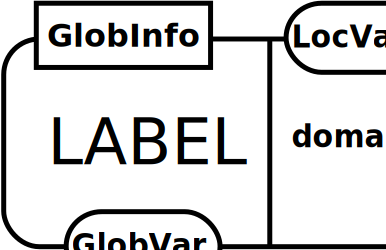
\includegraphics[scale = 0.3]{images/entity}
  \caption{The \ER glyph for \glyph{entity}.}
  \label{fig:entity}
\end{figure}

\normalcolor

% The following is for [X]Emacs users.   Please leave in place.
% Local Variables:
% TeX-master: "../sbgn_ER-level1"
% End:


%%%%%%%%%%%%%%%%%%%%%%%%%%%%%%%%%%%%%%%%%%%%%%%%%%%%%%%%%%%%%%%%%%%%%%
%%%%                   Outcome
%%%%%%%%%%%%%%%%%%%%%%%%%%%%%%%%%%%%%%%%%%%%%%%%%%%%%%%%%%%%%%%%%%%%%%
%\color{blue}
\subsubsection{Glyph: \glyph{Outcome}}\label{sec:outcome}

In \ERs, an \glyph{outcome} represents the actualisation of a \glyph{statement} (\sect{statements}). It is not entity on its own, but subset of all possible entity instances where \glyph{statement}  is true. For instance, if an \glyph{interaction} represents a non-covalent binding, the \glyph{outcome} represents all possible complexes that has two interactors bound to each other. If an \glyph{interaction} represents a genetic interaction, for instance derived from genetic screenings, the \glyph{outcome} represents the result of the presence of the two polymorphisms. If an \glyph{assignment} represents the phosphorylation of a protein, the \glyph{outcome} represents all possible complexes and free molecules where this protein is phosphorylated.

An \glyph{outcome} represent a particular instance of a realisation, and therefore, from one outcome must depart only one influence. An outcome being an \glyph{entity node}, it cannot receive influences. It exists. It cannot more or less exist. 

\begin{glyphDescription}

\glyphSboTerm SBO:0000409 ! interaction outcome

\glyphContainer  An \glyph{outcome} is represented by a black dot located on the arc of a \glyph{statement} (\sect{statements}). The diameter of the dot has to be larger than the thickness of the arc.

\glyphLabel An \glyph{outcome} has no identity on its own and does not carry any label. 

\glyphAux An \glyph{outcome} does not carry any auxiliary items.

\end{glyphDescription}

\begin{figure}[H]
  \centering
  \includegraphics[scale = 0.5]{images/outcome}
  \caption{The \ER glyph for \glyph{outcome}.}
  \label{fig:outcome}
\end{figure}

\begin{figure}[H]
  \centering
  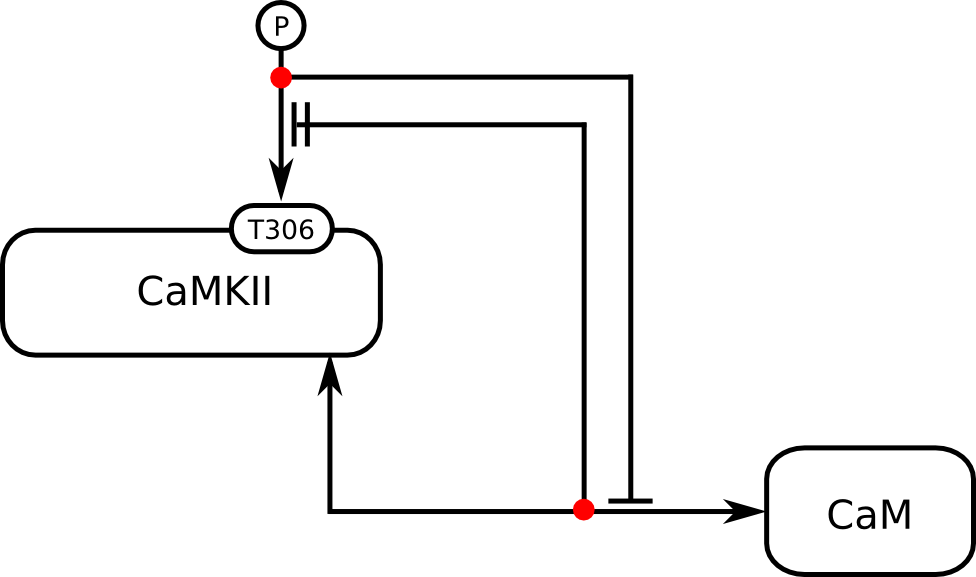
\includegraphics[scale = 0.5]{examples/ex-outcome}
  \caption{Examples of \glyph{outcomes}. The rightmost represents the fact that calmodulin effectively interacts (\sect{interaction}) with calcium/calmodulin kinase II. The leftmost represents the fact that the value phosphorylated is assigned (\sect{assignment}) to the variable representing threonin 306 of calcium/calmodulin kinase II.}
  \label{fig:ex-outcome}
\end{figure}

%\normalcolor
	


% %%%%%%%%%%%%%%%%%%%%%%%%%%%%%%%%%%%%%%%%%%%%%%%%%%%%%%%%%%%%%%%%%%%%%%
% %%%%%%%%%%%%%%%%%%%%%%%%%%%%%%%%%%%%%%%%%%%%%%%%%%%%%%%%%%%%%%%%%%%%%%
% %%%%                   Logical operators
% %%%%%%%%%%%%%%%%%%%%%%%%%%%%%%%%%%%%%%%%%%%%%%%%%%%%%%%%%%%%%%%%%%%%%%
% %%%%%%%%%%%%%%%%%%%%%%%%%%%%%%%%%%%%%%%%%%%%%%%%%%%%%%%%%%%%%%%%%%%%%%

\subsection{Logical operators}\label{sec:logic}

A \glyph{logical operator} allows to combine elements of truth into another element of truth (if A exists and B exits, then A AND B exists) in order ot apply influences. \SBGNERLone{} provides four \glyph{logical operators}, \glyph{and}, \glyph{or}, \glyph{not} and \glyph{delay}.

%%%%%%%%%%%%%%%%%%%%%%%%%%%%%%%%%%%%%%%%%%%%%%%%%%%%%%%%%%%%%%%%%%%%%%
%%                     And
%%%%%%%%%%%%%%%%%%%%%%%%%%%%%%%%%%%%%%%%%%%%%%%%%%%%%%%%%%%%%%%%%%%%%%
\color{blue}
\subsubsection{Glyph: \glyph{And}}\label{sec:and}

The glyph \glyph{and} is used to denote that all the \glyph{entity nodes} linked as input are necessary to produce the output influence.

\begin{glyphDescription}

 \glyphSboTerm SBO:0000173 ! and.

 \glyphContainer \glyph{And} is represented by a circle, with two connectors located at the opposite side for inputs and output.

  \glyphLabel \glyph{And} is identified by the label ``AND'' placed in an unbordered box attached to the center of the container. 

  \glyphAux \glyph{And} does not carry any auxiliary items.

\end{glyphDescription}


\begin{figure}[H]
  \centering
  \includegraphics[scale = 0.5]{images/and}
  \caption{The \ER glyph for \glyph{and}. Three inputs are represented, but two or more than three would be allowed.}
  \label{fig:and}
\end{figure}


% The following diagrams illustrate the dephosphorylation of the MAP inase ERK by the protein phosphatase 2A and the STriatal Enriched Phosphatase, in ST (left) and ER (right).
%
% \begin{center}
% \scalebox{0.5}{\includegraphics{images/stimulation-example1}}
% \end{center}
\normalcolor

%%%%%%%%%%%%%%%%%%%%%%%%%%%%%%%%%%%%%%%%%%%%%%%%%%%%%%%%%%%%%%%%%%%%%%
%%                     Or
%%%%%%%%%%%%%%%%%%%%%%%%%%%%%%%%%%%%%%%%%%%%%%%%%%%%%%%%%%%%%%%%%%%%%%
\color{blue}
\subsection{Glyph: \glyph{Or}}\label{sec:or}

The glyph \glyph{or} is used to denote that any of the \glyph{interactor nodes} linked as input is sufficient to produce the output influence.

\begin{glyphDescription}
 \glyphSboTerm SBO:0000174 ! or.
 \glyphOrigin One interactor (section~\ref{sec:interactors}) or logical operator (section~\ref{sec:logic}).
 \glyphTarget  One modulation (section~\ref{sec:modulation}), stimulation (section~\ref{sec:stimulation}), inhibition (section~\ref{sec:inhibition}), necessary  stimulation (section~\ref{sec:necessaryStimulation}), or absolute inhibition (section~\ref{sec:absoluteInhibition}) arc.
 \glyphNode \glyph{Or} is represented by a circle carrying the word ``OR''.
 \end{glyphDescription}

\begin{figure}[H]
  \centering
  \includegraphics[scale = 0.5]{images/or}
  \caption{The \ER glyph for \glyph{or}. Only two inputs are represented, but more would be allowed.}
  \label{fig:or}
\end{figure}



%%%%%%%%%%%%%%%%%%%%%%%%%%%%%%%%%%%%%%%%%%%%%%%%%%%%%%%%%%%%%%%%%%%%%%
%%                     Not
%%%%%%%%%%%%%%%%%%%%%%%%%%%%%%%%%%%%%%%%%%%%%%%%%%%%%%%%%%%%%%%%%%%%%%
\color{blue}
\subsubsection{Glyph: \glyph{Not}}\label{sec:not}

The glyph \glyph{not} is used to denote that the output influence only happen in the absence of the input \glyph{interactor}.

\begin{glyphDescription}

 \glyphSboTerm SBO:0000238 ! not.

 \glyphContainer \glyph{Not} is represented by a circle, with two connectors located at the opposite side for input and output.

  \glyphLabel \glyph{Not} is identified by the label ``NOT'' placed in an unbordered box attached to the center of the container. 

  \glyphAux \glyph{Not} does not carry any auxiliary items.

\end{glyphDescription}

\begin{figure}[H]
  \centering
  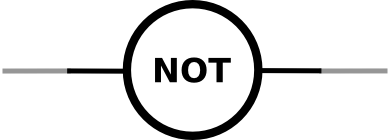
\includegraphics[scale = 0.5]{images/not}
  \caption{The \ER glyph for \glyph{not}.}
  \label{fig:not}
\end{figure}


%%%%%%%%%%%%%%%%%%%%%%%%%%%%%%%%%%%%%%%%%%%%%%%%%%%%%%%%%%%%%%%%%%%%%%
%%                     delay
%%%%%%%%%%%%%%%%%%%%%%%%%%%%%%%%%%%%%%%%%%%%%%%%%%%%%%%%%%%%%%%%%%%%%%
%\color{blue}
\subsubsection{Glyph: \glyph{delay}}\label{sec:delay}

The glyph \glyph{delay} is used to denote that the \glyph{entity nodes} linked as input does not produce the influence immediately, but a delay after the decision of influencing has been taken.

\begin{glyphDescription}

 \glyphSboTerm SBO:0000225 ! delay.

 \glyphContainer \glyph{Delay} is represented by a circle, with two connectors located at the opposite side for input and output.

  \glyphLabel \glyph{Delay} is identified by the greek letter ``$\tau$`` (``TAU'') placed in an unbordered box attached to the center of the container. 

  \glyphAux \glyph{Delay} does not carry any auxiliary items.

\end{glyphDescription}

\begin{figure}[H]
  \centering
  
\includegraphics[scale = 0.5]{images/delay}
  \caption{The \ER glyph for \glyph{delay}.}
  \label{fig:delay}
\end{figure}

\begin{figure}[H]
  \centering
  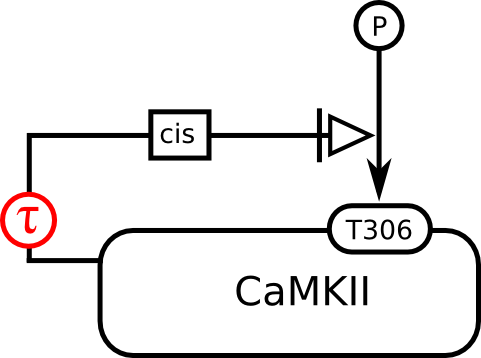
\includegraphics[scale = 0.5]{examples/ex-delay}
  \caption{Example of the \glyph{delay} logical operator, showing that the stimulation of the phosphorylation of CaMKII on threonin 306 takes place a measurable amount of time after the decision of stimulation is triggered.}
  \label{fig:ex-delay}
\end{figure}

%\normalcolor


% %%%%%%%%%%%%%%%%%%%%%%%%%%%%%%%%%%%%%%%%%%%%%%%%%%%%%%%%%%%%%%%%%%%%%%
% %%%%%%%%%%%%%%%%%%%%%%%%%%%%%%%%%%%%%%%%%%%%%%%%%%%%%%%%%%%%%%%%%%%%%%
% %%%%                   Perturbing agent
% %%%%%%%%%%%%%%%%%%%%%%%%%%%%%%%%%%%%%%%%%%%%%%%%%%%%%%%%%%%%%%%%%%%%%%
% %%%%%%%%%%%%%%%%%%%%%%%%%%%%%%%%%%%%%%%%%%%%%%%%%%%%%%%%%%%%%%%%%%%%%%

\subsection{Glyph: \glyph{Perturbing agent}}\label{sec:perturbation}
%%%%%%%%%%%%%%%%%%%%%%%%%%%%%%%%%%%%%%%%%%%%%%%%%%%%%%%%%%%%%%%%%%%%%%
%%                     Perturbing agent
%%%%%%%%%%%%%%%%%%%%%%%%%%%%%%%%%%%%%%%%%%%%%%%%%%%%%%%%%%%%%%%%%%%%%%
\color{red}

\subsection{Glyph: \glyph{Perturbing agent}}
\label{sec:perturbation}
 
Biochemical networks can be affected by external influences. Those
influences can be well-defined physical perturbations, such as a the effect of a light
pulse or of a change in temperature; they can also be more complex and not
well-defined phenomena, for instance a biological process, an experimental
setup, or a mutation.  For these situations, SBGN provides the
\glyph{perturbing agent} glyph. We do not use the word \emph{perturbation} to avoid the misunderstanding with the influence that the \glyph{perturbing agent} has on the map. 

\begin{glyphDescription}

\glyphSboTerm SBO:0000405 ! perturbing agent

\glyphContainer A \glyph{perturbing agent} is represented by a modified hexagon
having two opposite concave faces, as illustrated in \fig{perturbation}.

\glyphLabel A \glyph{perturbing agent} is identified by a label placed in an
unbordered box containing a string of characters.  The characters can be
distributed on several lines to improve readability, although this is not
mandatory.  The label box must be attached to the center of the
\glyph{perturbing agent} container.  The label may spill outside of the container.

\glyphAux A \glyph{perturbing agent} does not carry any auxiliary unit. [DOES-IT NOT? IS-IT AN ENTRY POINT? WHAT ABOUT THE EXISTENCE AND LOCATION VARIABLES?]

\end{glyphDescription}

\begin{figure}[H]
  \centering
  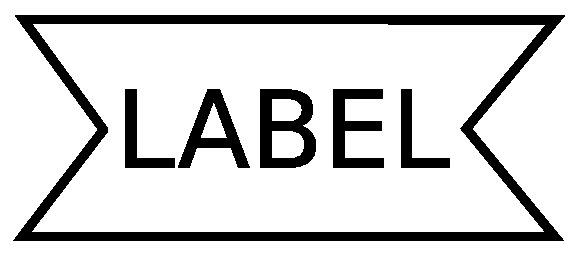
\includegraphics[scale = 0.3]{images/perturbation}
  \caption{The \ER glyph for \glyph{perturbing agent}.}
  \label{fig:perturbation}
\end{figure}

\begin{figure}[H]
  \centering
  \includegraphics[scale = 0.5]{examples/ex-perturbing}
  \caption{Example of a \glyph{perturbing agent} representing the depolarisation of a membrane, that stimulates (\sect{stimulation}) the existence (see \ref{sec:existence}) of an interactor.}
  \label{fig:ex-perturbing}
\end{figure}

\normalcolor


%%%%%%%%%%%%%%%%%%%%%%%%%%%%%%%%%%%%%%%%%%%%%%%%%%%%%%%%%%%%%%%%%%%%%%
%%%%%%%%%%%%%%%%%%%%%%%%%%%%%%%%%%%%%%%%%%%%%%%%%%%%%%%%%%%%%%%%%%%%%%
%%%%                   Relationship arcs
%%%%%%%%%%%%%%%%%%%%%%%%%%%%%%%%%%%%%%%%%%%%%%%%%%%%%%%%%%%%%%%%%%%%%%
%%%%%%%%%%%%%%%%%%%%%%%%%%%%%%%%%%%%%%%%%%%%%%%%%%%%%%%%%%%%%%%%%%%%%%

\section{Relationships}\label{sec:relationships}

\glyph{Relationships} are rules that decide of the existence of entity nodes, based on the existence of others. 
%In ontology parlance, they would be ``occurants''. 
\SBGNERLone{} provides two types of relationships, the statements and the influences.

%%%%%%%%%%%%%%%%%%%%%%%%%%%%%%%%%%%%%%%%%%%%%%%%%%%%%%%%%%%%%%%%%%%%%%
%%%%%%%%%%%%%%%%%%%%%%%%%%%%%%%%%%%%%%%%%%%%%%%%%%%%%%%%%%%%%%%%%%%%%%
%%%%                   Statements
%%%%%%%%%%%%%%%%%%%%%%%%%%%%%%%%%%%%%%%%%%%%%%%%%%%%%%%%%%%%%%%%%%%%%%
%%%%%%%%%%%%%%%%%%%%%%%%%%%%%%%%%%%%%%%%%%%%%%%%%%%%%%%%%%%%%%%%%%%%%%

\subsection{Statements}\label{sec:statements}

\glyph{Statements} can be true or false. \glyph{Statements} are targets of \glyph{influences}. They are not true themselves, but can carry truth element (\glyph{outcomes}, see \sect{outcome}). \SBGNERLone{} provides three types of statements, \glyph{assignment}, \glyph{interaction} and \glyph{phenotype}.

%%%%%%%%%%%%%%%%%%%%%%%%%%%%%%%%%%%%%%%%%%%%%%%%%%%%%%%%%%%%%%%%%%%%%%
%%                    Assignment
%%%%%%%%%%%%%%%%%%%%%%%%%%%%%%%%%%%%%%%%%%%%%%%%%%%%%%%%%%%%%%%%%%%%%%
%\color{blue}

\subsubsection{Glyph: \glyph{Assignment}}\label{sec:assignment}

\glyph{Assignment} is used to describe the setting of a state variable to a certain value. The assignment, represented by an harpoon arrow, goes from on or more variable values, represented by floating \glyph{state variables} to a variable identification, represented by a \glyph{state variable} attached to the entity affected by the assignment. If an \glyph{assignment} take several \glyph{state variable} values are input, there is an implicit XOR between them. Only one value can be assigned at a time. The result of an assignment is represented by \glyph{outcomes}, that is by filled dots on the arrow. The result of an \glyph{assignment} can be represented by any number of \glyph{outcomes}. In the case of more than one \glyph{state variable} values, the \glyph{outcomes} must be placed on the relevant incoming branch.

\begin{glyphDescription}
 \glyphSboTerm non-applicable
 \glyphOrigin One or more state-variables (section \sect{stateVariable}) on their own, each containing a variable value.
 \glyphTarget A state-variable (section \sect{stateVariable}) carried by a interactor (section \sect{interactors}), containing a variable identification.
 \glyphEndPoint The target extremity of an \glyph{assignment} carries an harpoon arrowhead.
 \end{glyphDescription}

\begin{figure}[H]
  \centering
  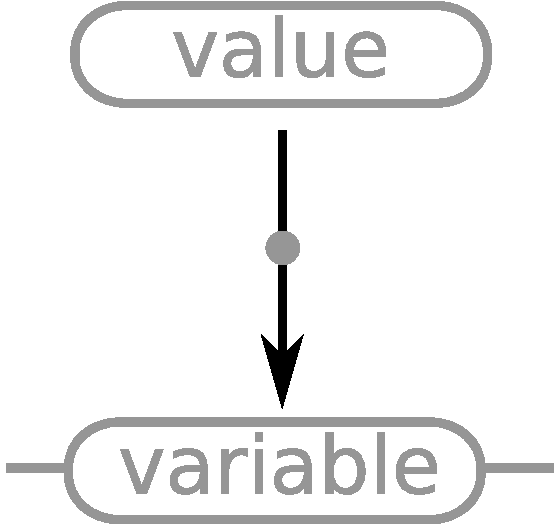
\includegraphics[scale = 0.3]{images/assignment}
  \caption{The \ER glyph for \glyph{assignment}.}
  \label{fig:assignment}
\end{figure}

\begin{figure}[H]
  \centering
  \includegraphics[scale = 0.5]{examples/ex-assignment}
  \caption{Two examples of \glyph{assignment} representing phosphorylation, by one value (phosphorylation) of a variable representing a residue, or two values (true or false) of a variable representing the phosphorylated residue.}
  \label{fig:ex-assignment}
\end{figure}


%\normalcolor

%%%%%%%%%%%%%%%%%%%%%%%%%%%%%%%%%%%%%%%%%%%%%%%%%%%%%%%%%%%%%%%%%%%%%%
%%                    Interaction
%%%%%%%%%%%%%%%%%%%%%%%%%%%%%%%%%%%%%%%%%%%%%%%%%%%%%%%%%%%%%%%%%%%%%%
%\color{blue}

\subsubsection{Glyph: \glyph{Interaction}}\label{sec:interaction}

\glyph{Interaction} represents an interaction between two or more \glyph{entities} or \glyph{outcomes}, whether a non-covalent physical interaction, or a functional interaction, e.g. genetic interaction. The interaction is represented by a circle which connect to arrows pointing to the interactors involved in the interaction. In the case of a binary interaction, the circle may be ommitted. The realisation of the interaction is represented by \glyph{outcomes} (see section \ref{sec:outcome}), that is by filled dots. These \glyph{outcomes} are located on the circle representing the interaction. In the case of a binary interaction represented without circle, the \glyph{outcomes} can be placed anywhere between the arrowheads. The realisations of an interaction can be represented by any number of \glyph{outcomes}. The \glyph{influences} (\ref{sec:influences}) targeting an interaction end up on the external side of the circle, between the \glyph{outcomes}.

\begin{glyphDescription}
 \glyphSboTerm SBO:0000342 molecular or genetic interaction
 \glyphOrigin Any \glyph{interactor} (\sect{interactors}).
 \glyphTarget Any \glyph{interactor} (\sect{interactors}).
 \glyphEndPoint Both origin and target extremities of an \glyph{interaction} carry an harpoon arrowhead. The arrows pointing to the \glyph{interactors} originate from a circle. In the case of a binary interaction, the circle is optional. 
\glyphAux A \glyph{unit of information} containing a \glyph{cardinality} (\sect{miscellaneous-cv}) indicates the number of instances of an entity involved in an interaction. The absence of a \glyph{cardinality} is synonymous of a cardinality of 1. A \glyph{unit of information} on a binary interaction involving only one entity, or outcomes of interactions involving one entity, carrying the mention \glyph{cis} or \glyph{trans} precises if the interaction is intra-molecular or between different instances of the same entity or complex.
 \end{glyphDescription}

\begin{figure}[H]
  \centering
  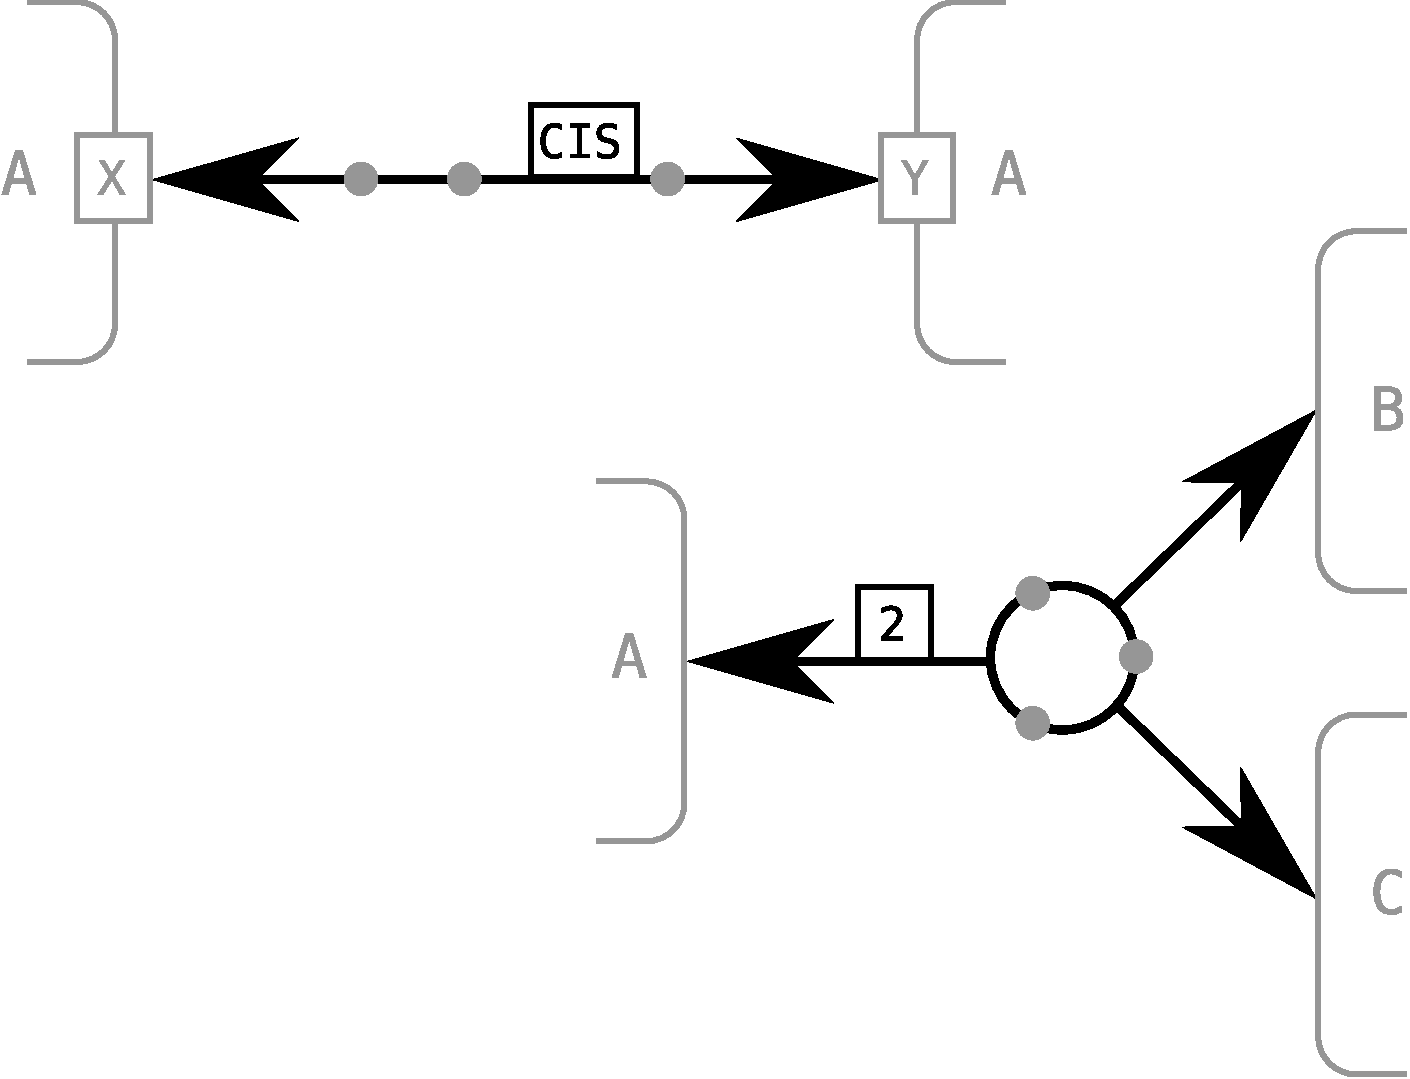
\includegraphics[scale = 0.3]{images/interaction}
  \caption{The \ER glyph for \glyph{interaction}. Top left, binary interaction between two entities. The circle can be ommitted, and the \glyph{outcomes} located anywhere on the \glyph{interaction}. Bottom left, because the cardinality of the entity A is 2, the interaction is not a binary one, but a n-ary one. The circle cannot be ommitted. Bottom right, n-ary interaction with three different entities. Top right, intra-molecular interaction; }
  \label{fig:interaction}
\end{figure}

\begin{figure}[H]
  \centering
  \includegraphics[scale = 0.5]{examples/ex-interaction}
  \caption{Examples of \glyph{interactions}, showing the effect of the binding of calmodulin to CaMKII (binary interaction) on the folding of the kinase (intra-molecular interaction), and the effect of the folding or the dimerisation of CaMKII (inter-molecular interaction between different instances of CaMKII) on the binding of calmodulin.}
  \label{fig:ex-interaction}
\end{figure}

\begin{figure}[H]
  \centering
  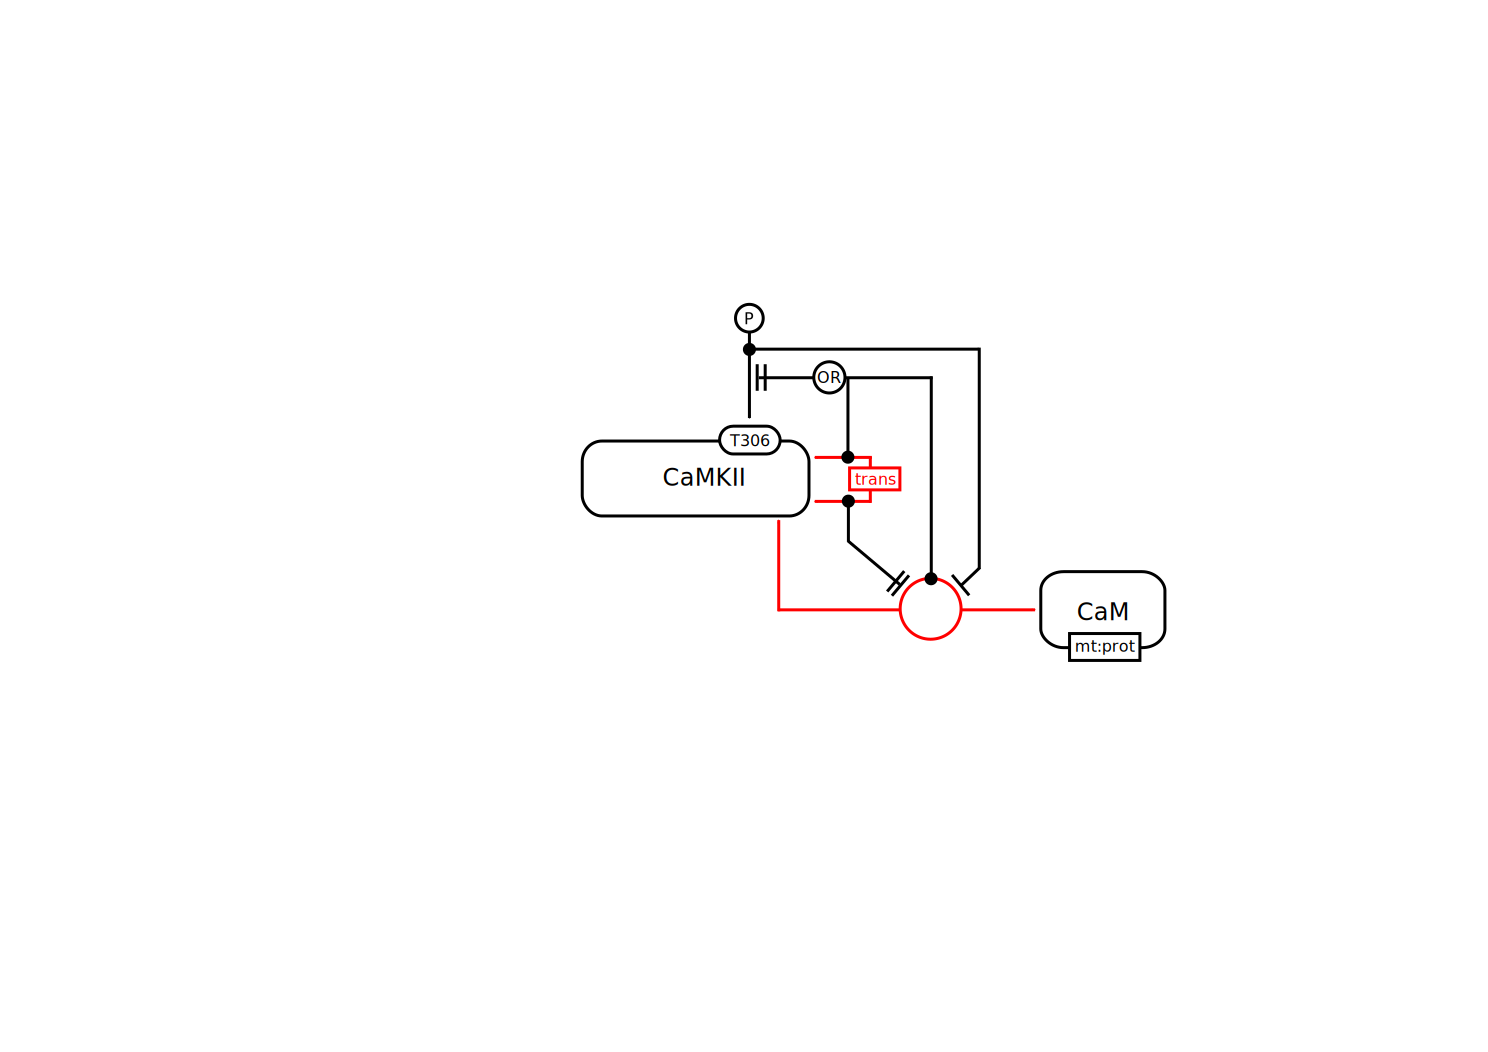
\includegraphics[scale = 0.5]{examples/ex-interaction-influences}
  \caption{Examples of a binary \glyph{interaction} between CaMKII and calmodulin where the interaction is represented by a circle. Interaction between adjacent monomers of CaMKII (trans-interaction) preclude the binding of calmodulin, as represented by an \glyph{absolute inhibition} ending on the circle. The phosphorylation of threonine 306 also inhibits the interaction. The realisation of the interaction, represented by an \glyph{outcome} located on the circle, itself inhibits the phosphorylation of threonine 306.}
  \label{fig:ex-interaction-influences}
\end{figure}
%\normalcolor
%%%%%%%%%%%%%%%%%%%%%%%%%%%%%%%%%%%%%%%%%%%%%%%%%%%%%%%%%%%%%%%%%%%%%%%
%%                    Non-Interaction
%%%%%%%%%%%%%%%%%%%%%%%%%%%%%%%%%%%%%%%%%%%%%%%%%%%%%%%%%%%%%%%%%%%%%%
\color{red}

\subsubsection{Glyph: \glyph{Non-Interaction}}\label{sec:non-interaction}

\glyph{Non-interaction} represents the absence of an interaction between two or more \glyph{entities} or \glyph{outcomes}, whether a non-covalent physical interaction, or a functional interaction, e.g. genetic interaction. Each arrowhead points to an interactor involved in the absent interaction. The result of the non-interaction is represented by \glyph{outcomes} (see section \ref{sec:outcome}), that is by filled dots on the line linking the two arrowheads in the case of a binary interaction, on a circle linked to the edges coming from the arrowheads in the case of a  n-ary interactions. The result of an interaction can be represented by any number of \glyph{outcomes}.

\begin{glyphDescription}
 \glyphSboTerm SBO:NEW
 \glyphOrigin Any \glyph{interactor} (\sect{interactors}).
 \glyphTarget Any \glyph{interactor} (\sect{interactors}).
 \glyphEndPoint Both origin and target extremities of a \glyph{non-interaction} carry an harpoon arrowhead. In the case of n-ary non-interactions, the arrows pointing to the \glyph{interactors} originate from a circle. 
 \glyphAux A \glyph{unit of information} containing a \glyph{cardinality} (\sect{miscellaneous-cv}) indicates the number of instances of an entity involved in an interaction. A \glyph{unit of information} on a binary non-interaction involving only one entity carrying the mention \glyph{cis} or \glyph{trans} precises if this is an absence of an intra-molecular interaction or and interaction between different instances of the same entity.
 \end{glyphDescription}

\begin{figure}[H]
  \centering
  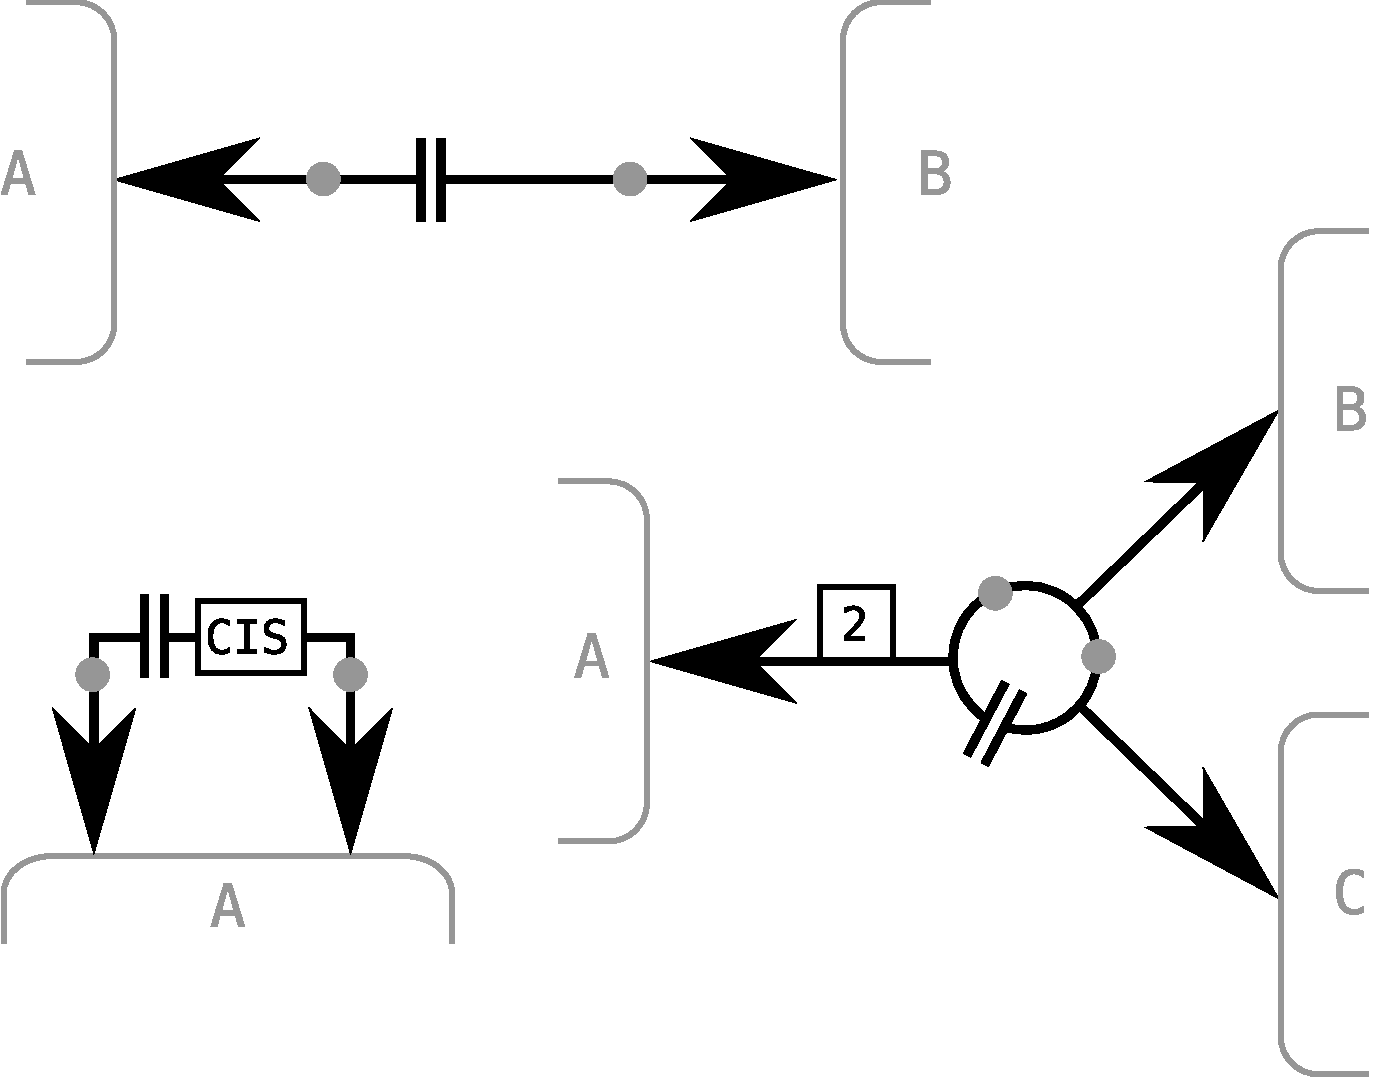
\includegraphics[scale = 0.3]{images/non-interaction}
  \caption{The \ER glyph for \glyph{non-interaction}. Top, binary non-interaction between two entities; bottom left, absence of an intra-molecular interaction; bottom right, absence of an n-ary interaction.}
  \label{fig:non-interaction}
\end{figure}

\normalcolor

\color{ForestGreen}

\subsection{Glyph: \glyph{Phenotype}}
\label{sec:phenotype}

A biochemical network can generate phenotypes or affect biological
processes.  Such processes can take place at different levels and are
independent of the biochemical network itself.  To represent these
processes in a diagram, SBGN defines the \glyph{phenotype} glyph.

\begin{glyphDescription}

\glyphSboTerm SBO:0000358 ! phenotype
\glyphOrigin Non-applicable
\glyphTarget Non-applicable
\glyphEndPoint A \glyph{phenotype} is represented by an elongated
hexagon, as illustrated in \fig{phenotype}. It is identified by a label placed in an
unbordered box containing a string of characters.  The characters can be
distributed on several lines to improve readability, although this is not
mandatory.  The label box must be attached to the center of the
\glyph{phenotype} container.  The label may spill outside of the container.

\end{glyphDescription}
 
\begin{figure}[H]
  \centering
  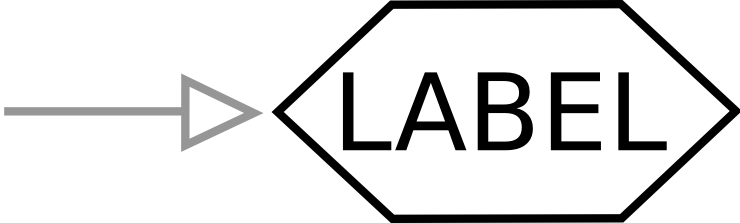
\includegraphics[scale = 0.3]{images/phenotype}
  \caption{The \ER glyph for \glyph{phenotype}.}
  \label{fig:phenotype}
\end{figure}

\begin{figure}[H]
  \centering
  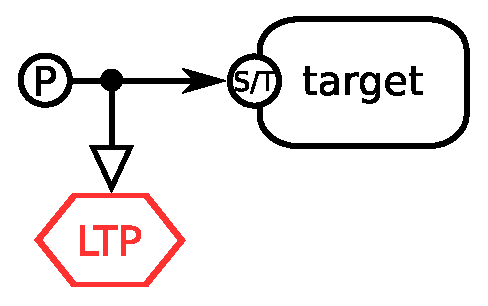
\includegraphics[scale = 0.5]{examples/ex-phenotype}
  \caption{Example of a \glyph{phenotype} ``Long Term Potentiation (LTP)'' enhanced when the entity ``GluR'' is present in the post-synaptic density.}
  \label{fig:ex-phenotype}
\end{figure}

\normalcolor


\subsection{Influences}\label{sec:influences}

Influence arcs represent the effect of an entity on another relationship. The symbols attached to their extremities precise their semantics. SBGN \ERs{}' influences can be viewed as logical rules linking \glyph{ENs} and other rules. \SBGNERLone{} provides seven influences, \glyph{modulation}, \glyph{stimulation}, \glyph{inhibition}, \glyph{necessaryStimulation}, \glyph{absoluteInhibition}, \glyph{absoluteStimulation}, \glyph{logicArc}.

%%%%%%%%%%%%%%%%%%%%%%%%%%%%%%%%%%%%%%%%%%%%%%%%%%%%%%%%%%%%%%%%%%%%%%
%%                     Modulation
%%%%%%%%%%%%%%%%%%%%%%%%%%%%%%%%%%%%%%%%%%%%%%%%%%%%%%%%%%%%%%%%%%%%%%
\color{blue}
\subsubsection{Glyph: \glyph{Modulation}}\label{sec:modulation}

A modulation affects the strength, or the probability to exist, of the target relationship. Such a modulation can affect the relationship \textbf{positively or negatively}, or even both ways depending on the conditions. A \glyph{modulation} can also be used when one does not know the precise direction of the effect, for instance if there are conflicting evidence.

\begin{glyphDescription}
 \glyphSboTerm SBO:0000168 ! control.
 \glyphOrigin Any \glyph{entity node} (\sect{ENs}).
 \glyphTarget Any \glyph{relationship} (\sect{relationships}).
 \glyphEndPoint The target extremity of a \glyph{modulation} carries an empty diamond.
 \end{glyphDescription}

\begin{figure}[H]
  \centering
  
\includegraphics[scale = 0.5]{images/modulation}
  \caption{The \ER glyph for \glyph{modulation}.}
  \label{fig:modulation}
\end{figure}
 
\begin{figure}[H]
  \centering
  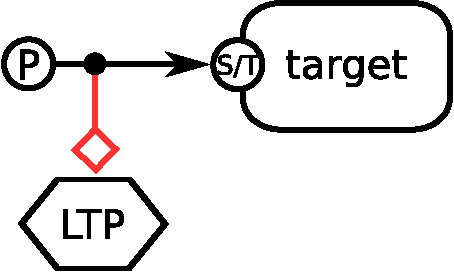
\includegraphics[scale = 0.5]{examples/ex-modulation}
  \caption{Example of a \glyph{modulation} of the \glyph{phenotype} ``Long Term Potentiation (LTP)'' by the phosphorylation of an \glyph{entity} ``target''. For instance the influence could be positive (stimulation, see \sect{stimulation}) or negative (inhibition, see \sect{inhibition}).}
  \label{fig:ex-modulation}
\end{figure}

\normalcolor


%%%%%%%%%%%%%%%%%%%%%%%%%%%%%%%%%%%%%%%%%%%%%%%%%%%%%%%%%%%%%%%%%%%%%%
%%                     Stimulation
%%%%%%%%%%%%%%%%%%%%%%%%%%%%%%%%%%%%%%%%%%%%%%%%%%%%%%%%%%%%%%%%%%%%%%

\subsubsection{Glyph: \glyph{Stimulation}}\label{sec:stimulation}
\color{blue}

A \glyph{stimulation} affects \textbf{positively} the strength, or the probability, of the target relationship. This stimulation can be for instance a catalysis or a positive allosteric regulation.

\begin{glyphDescription}
 \glyphSboTerm SBO:0000170 ! stimulation.
 \glyphOrigin Any \glyph{entity node} (\sect{ENs}).
 \glyphTarget Any \glyph{relationship} (\sect{relationships}).
 \glyphEndPoint The target extremity of a \glyph{stimulation} carries an empty arrowhead.
 \glyphAux A \glyph{unit of information} carrying the mention \glyph{cis} or \glyph{trans} precises the relationship between the \glyph{entity node} from which the \glyph{stimulation} origins and either:
\begin{itemize}
\item the \glyph{entity node} from which the influence targeted by the \glyph{stimulation} origins
\item all the relevant \glyph{interactors} of the \glyph{interaction} or the \glyph{non-interaction} targeted by the \glyph{stimulation}
\item the \glyph{entity} subjected to the \glyph{assignment} targeted by the \glyph{stimulation}
\end{itemize}
 \end{glyphDescription}

\begin{figure}[H]
  \centering
  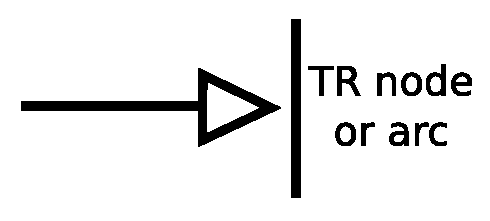
\includegraphics[scale = 0.5]{images/stimulation}
  \caption{The \PD glyph for \glyph{stimulation}.}
  \label{fig:stimulation}
\end{figure}

\begin{figure}[H]
  \centering
  \includegraphics[scale = 0.5]{examples/ex-stimulation}
  \caption{Example of a \glyph{stimulation} a \glyph{phenotype} ``Long Term Potentiation (LTP)'' enhanced when the entity ``GluR'' is present in the post-synaptic density.}
  \label{fig:ex-stimulation}
\end{figure}

\normalcolor




%%%%%%%%%%%%%%%%%%%%%%%%%%%%%%%%%%%%%%%%%%%%%%%%%%%%%%%%%%%%%%%%%%%%%%
%%                     Inhibition
%%%%%%%%%%%%%%%%%%%%%%%%%%%%%%%%%%%%%%%%%%%%%%%%%%%%%%%%%%%%%%%%%%%%%%

\subsubsection{Glyph: \glyph{Inhibition}}\label{sec:inhibition}
\color{blue}

An inhibition \textbf{negatively}  the strength, or the probability, of the target relationship. This inhibition can be for instance a steric hindrance or a negative allosteric regulation.

\begin{glyphDescription}
 \glyphSboTerm SBO:0000170 ! inhibition.
 \glyphOrigin Any \glyph{entity node} (\sect{ENs}).
 \glyphTarget Any \glyph{relationship} (\sect{relationships}).
 \glyphEndPoint The target extremity of a \glyph{inhibition} carries a bar perpendicular to the arc.
 \end{glyphDescription}

\begin{figure}[H]
  \centering
  \includegraphics[scale = 0.3]{images/inhibition}
  \caption{The \PD glyph for \glyph{inhibition}.}
  \label{fig:inhibition}
\end{figure}

\begin{figure}[H]
  \centering
  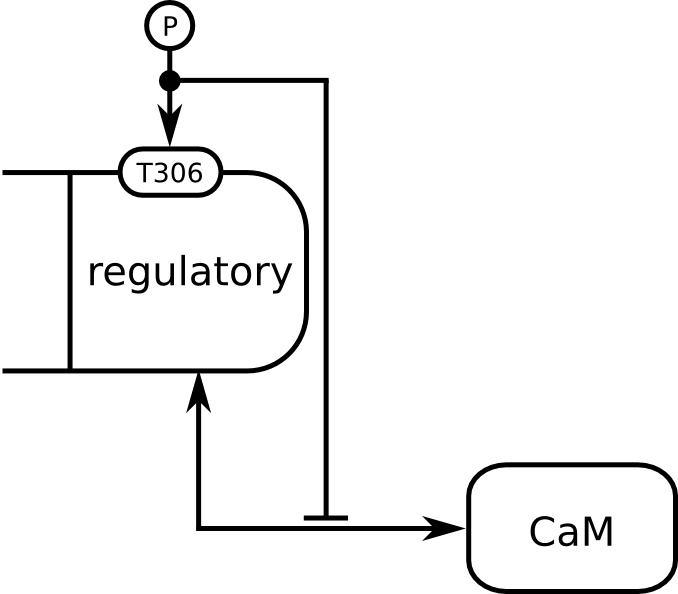
\includegraphics[scale = 0.5]{examples/ex-inhibition}
  \caption{In this example, the phosphorylation of the threonine 306 of the regulatory domain of CaMKII inhibits the interaction between Calmodulin and the kinase.}
  \label{fig:ex-inhibition}
\end{figure}

\normalcolor


%%%%%%%%%%%%%%%%%%%%%%%%%%%%%%%%%%%%%%%%%%%%%%%%%%%%%%%%%%%%%%%%%%%%%%
%%                     necessary stimulation
%%%%%%%%%%%%%%%%%%%%%%%%%%%%%%%%%%%%%%%%%%%%%%%%%%%%%%%%%%%%%%%%%%%%%%
%\color{blue}

\subsubsection{Glyph: \glyph{Necessary stimulation}}\label{sec:necessaryStimulation}

A \glyph{necessary stimulation} is an influence that has to be present for a relationship to take place (to become true). A relationship modulated by a necessary stimulation can only exist when this stimulation is true, whatever are the other influences this relationship is subjected to.

\begin{glyphDescription}
 \glyphSboTerm SBO:0000171 ! necessary stimulation.
 \glyphOrigin Any \glyph{entity node} (\sect{ENs}).
 \glyphTarget Any \glyph{relationship} (\sect{relationships}).
 \glyphEndPoint The target extremity of a \glyph{necessary stimulation} carries an open arrow (to remind that it is a \glyph{stimulation}) coming after a larger vertical bar.
 \glyphAux A \glyph{unit of information} carrying the mention \glyph{cis} or \glyph{trans} precises the relationship between the \glyph{entity node} from which the \glyph{necessary stimulation} origins and either:
\begin{itemize}
\item the \glyph{entity node} from which the influence targeted by the \glyph{necessary stimulation} origins
\item all the relevant \glyph{interactors} of the \glyph{interaction} targeted by the \glyph{necessary stimulation}
\item the \glyph{entity} subjected to the \glyph{assignment} targeted by the \glyph{necessary stimulation}
\end{itemize}

 \end{glyphDescription}

\begin{figure}[H]
  \centering
  
\includegraphics[scale = 0.5]{images/necessaryStimulation}
  \caption{The \ER glyph for \glyph{necessaryStimulation}.}
  \label{fig:necessaryStimulation}
\end{figure}

\begin{figure}[H]
  \centering
  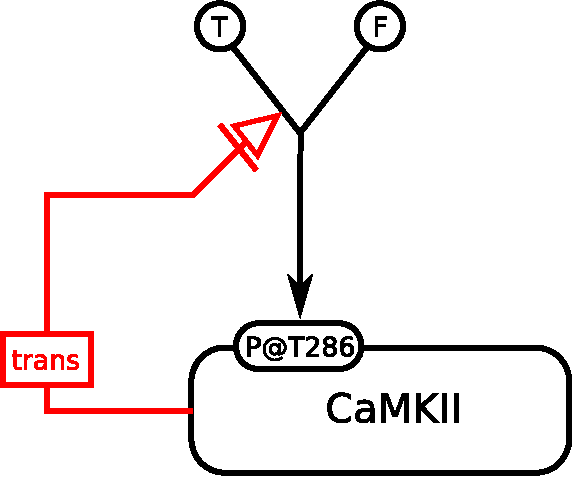
\includegraphics[scale = 0.5]{examples/ex-necessaryStimulation}
  \caption{This example shows how threonine 286 of CaMKII is only phosphorylated by the kinase itself, but in a trans-fashion, meaning a molecule of CaMKII does not phosphorylate itself, but another molecule of CaMKII.}
  \label{fig:ex-necessaryStimulation}
\end{figure}

%\normalcolor
%%%%%%%%%%%%%%%%%%%%%%%%%%%%%%%%%%%%%%%%%%%%%%%%%%%%%%%%%%%%%%%%%%%%%%
%%                     absolute stimulation
%%%%%%%%%%%%%%%%%%%%%%%%%%%%%%%%%%%%%%%%%%%%%%%%%%%%%%%%%%%%%%%%%%%%%%
\color{red}

\subsubsection{Glyph: \glyph{Absolute inhibition}}\label{sec:absoluteInhibition}

An absolute inhibition precludes the existence of another relationship. A relationship modulated by an absolute inhibition can only exist when an absolute inhibition in false, whatever are the other influences this relationship is subjected to.

\begin{glyphDescription}
 \glyphSboTerm SBO:0000171 ! absolute inhibition.
 \glyphOrigin Any \glyph{entity node} (\sect{ENs}).
 \glyphTarget Any \glyph{relationship} (\sect{relationships}).
 \glyphEndPoint The target extremity of a \glyph{absolute inhibition} carries a double bar perpendicular to the arc (to remind that it is an \glyph{inhibition}).
 \end{glyphDescription}

\begin{figure}[H]
  \centering
  
\includegraphics[scale = 0.5]{images/absoluteInhibition}
  \caption{The \PD glyph for \glyph{absoluteInhibition}.}
  \label{fig:absoluteInhibition}
\end{figure}

\begin{figure}[H]
  \centering
  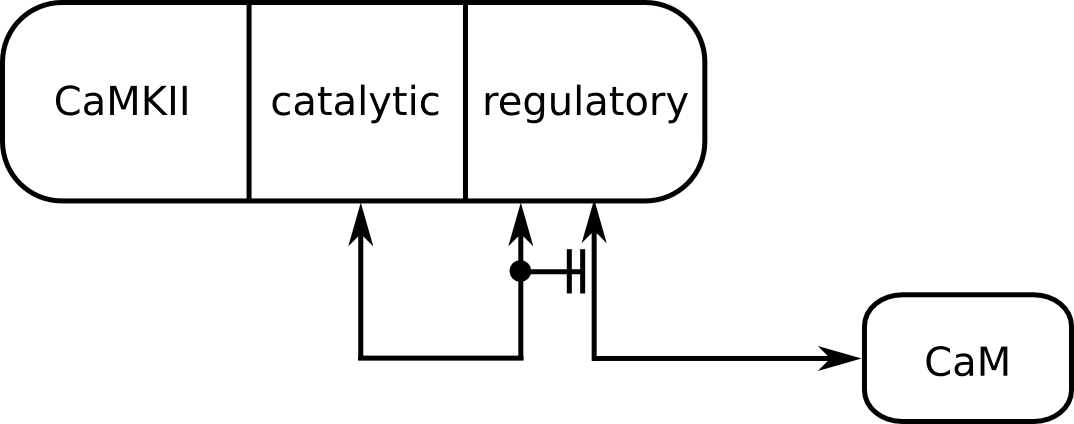
\includegraphics[scale = 0.5]{examples/ex-absoluteInhibition}
  \caption{This example shows how an intra-molecular interaction between catalytic and regulatory domains of CaMKII precludes totally the interaction of Calmodulin with CaMKII.}
  \label{fig:ex-absoluteInhibition}
\end{figure}

\normalcolor
%%%%%%%%%%%%%%%%%%%%%%%%%%%%%%%%%%%%%%%%%%%%%%%%%%%%%%%%%%%%%%%%%%%%%%
%%                     absolute stimulation
%%%%%%%%%%%%%%%%%%%%%%%%%%%%%%%%%%%%%%%%%%%%%%%%%%%%%%%%%%%%%%%%%%%%%%
\color{red}

\subsubsection{Glyph: \glyph{Absolute stimulation}}\label{sec:absoluteStimulation}

An absolute stimulation always trigger the existence of a target relationship. 

\begin{glyphDescription}
 \glyphSboTerm SBO:0000411 ! absolute stimulation
 \glyphOrigin Any \glyph{entity node} (\sect{ENs}).
 \glyphTarget Any \glyph{relationship} (\sect{relationships}).
 \glyphEndPoint The target extremity of a \glyph{absolute inhibition} carries a double empty arrowhead (to remind that it is a \glyph{stimulation}).
 \end{glyphDescription}

\begin{figure}[H]
  \centering
  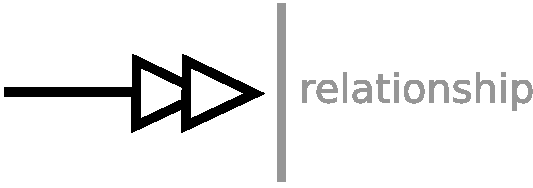
\includegraphics[scale = 0.5]{images/absoluteStimulation}
  \caption{The \PD glyph for \glyph{absoluteStimulation}.}
  \label{fig:absoluteStimulation}
\end{figure}


\normalcolor
%%%%%%%%%%%%%%%%%%%%%%%%%%%%%%%%%%%%%%%%%%%%%%%%%%%%%%%%%%%%%%%%%%%%%%
%%                     Logic arc
%%%%%%%%%%%%%%%%%%%%%%%%%%%%%%%%%%%%%%%%%%%%%%%%%%%%%%%%%%%%%%%%%%%%%%
%\color{blue}
\subsubsection{Glyph: \glyph{Logic arc} }\label{sec:logicArc}

\glyph{Logic arc} is used to represent the fact that an interactor influences
the outcome of a logic operator. 

\begin{glyphDescription}
 \glyphSboTerm SBO:0000398 - logical relationship.
 \glyphOrigin Any \glyph{interactor} (\sect{interactors}) or \glyph{logical operator} (\sect{logic}).
 \glyphTarget Any \glyph{logical operator} (\sect{logic}).
 \glyphEndPoint No particular symbol is used to represent a logic arc.
 \end{glyphDescription}

\begin{figure}[H]
  \centering
  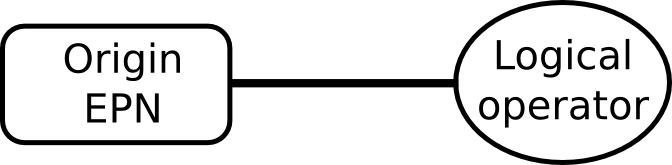
\includegraphics[scale = 0.4]{images/logicArc}
  \caption{The \ER glyph for \glyph{logic arc}.}
  \label{fig:logicArc}
\end{figure}

\begin{figure}[H]
  \centering
  \includegraphics[scale = 0.5]{examples/ex-logicArc}
  \caption{In this example, two logic arcs reflect the fact that the phosphorylation of threonine 306 on CaMKII is precluded either by a dimerisation or the binding of calmodulin.}
  \label{fig:ex-logicArc}
\end{figure}

%\normalcolor

%\section{Submap}\label{sec:submap}
%%%%%%%%%%%%%%%%%%%%%%%%%%%%%%%%%%%%%%%%%%%%%%%%%%%%%%%%%%%%%%%%%%%%%%%
%%%%                   Submap
%%%%%%%%%%%%%%%%%%%%%%%%%%%%%%%%%%%%%%%%%%%%%%%%%%%%%%%%%%%%%%%%%%%%%%

\color{red}

A \glyph{submap} is used to encapsulate entities and relationships (including all types of nodes and edges) within one named glyph. The content of the submap can be found for instance on another (web) page in the case of static maps, or can be displayed dynamicaly. Because of the independence of rules, no particular connections are needed between the submap and the containing map.

\begin{figure}[H]
  \centering
  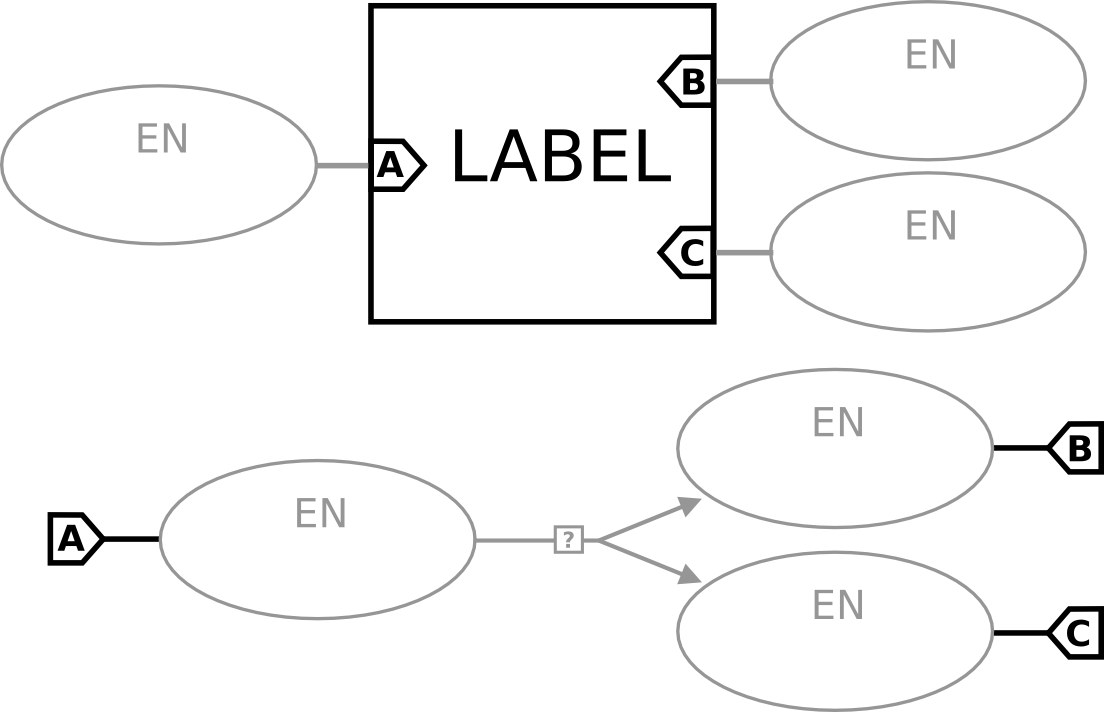
\includegraphics[scale = 0.3]{images/submap}
  \caption{The \ER glyph for \glyph{submap}.}
  \label{fig:submap}
\end{figure}


\normalcolor


%%%%%%%%%%%%%%%%%%%%%%%%%%%%%%%%%%%%%%%%%%%%%%%%%%%%%%%%%%%%%%%%%%%%%%
%%                     Annotation
%%%%%%%%%%%%%%%%%%%%%%%%%%%%%%%%%%%%%%%%%%%%%%%%%%%%%%%%%%%%%%%%%%%%%%
%\color{red}

\section{Glyph: \glyph{Annotation}}
\label{sec:annotation}


\SBGNERLone defines a glyph to add additional information to a map, that does not modify the semantic of the the graph. This glyph can be used to add free text, or links to external information.

\begin{glyphDescription}

\glyphSboTerm SBO:NEW

\glyphContainer An \glyph{annotation} is represented by a rectangular container with a folded corner, as illustrated in \fig{annotation}. This container is linked to the annotated element with a callout. The link ends up on the border of the annotated element.

\glyphLabel An \glyph{annotation} contains information placed in an unbordered box containing a string of characters.  The characters can be distributed on several lines to improve readability, although this is not mandatory.  The label box must be attached to the center of the container. The label may spill outside of the container. 

\glyphAux An \glyph{annotation} does not carry any auxiliary unit.
\end{glyphDescription}

\begin{figure}[H]
  \centering
  
\includegraphics[scale = 0.3]{images/annotation}
  \caption{The \ER glyph for \glyph{annotation}.}
  \label{fig:annotation}
\end{figure}

\begin{figure}[H]
  \centering
  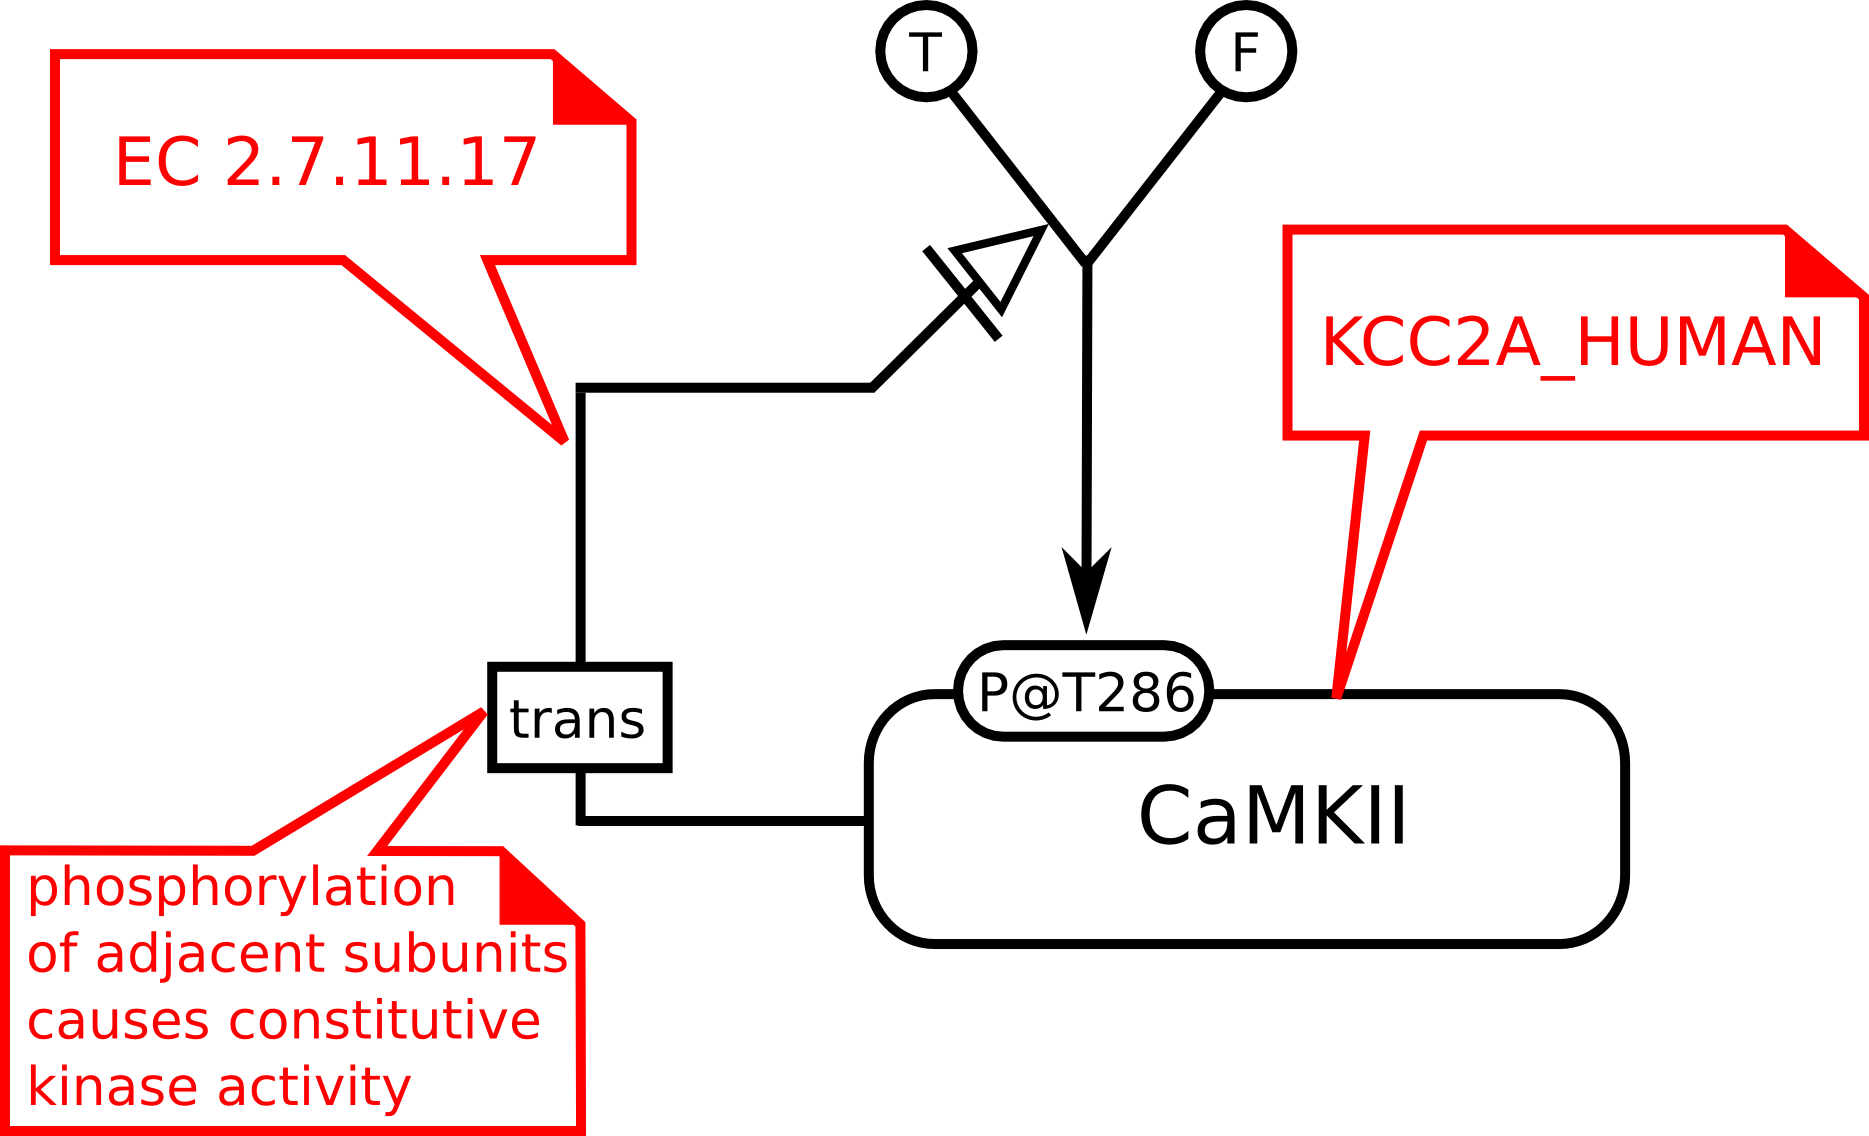
\includegraphics[scale = 0.5]{examples/ex-annotation}
  \caption{Example of \glyph{annotations} adding information to the description of the trans-phosphorylation of CaMKII. Note that three different types of links are used between annotation nodes and annotated elements. However, it is recommended to use a consistent scheme whithin a map.}
  \label{fig:ex-annotation}
\end{figure}

%\normalcolor


% %%%%%%%%%%%%%%%%%%%%%%%%%%%%%%%%%%%%%%%%%%%%%%%%%%%%%%%%%%%%%%%%%%%%%%
% %%%%%%%%%%%%%%%%%%%%%%%%%%%%%%%%%%%%%%%%%%%%%%%%%%%%%%%%%%%%%%%%%%%%%%
% %%%%                   Auxiliary units
% %%%%%%%%%%%%%%%%%%%%%%%%%%%%%%%%%%%%%%%%%%%%%%%%%%%%%%%%%%%%%%%%%%%%%%
% %%%%%%%%%%%%%%%%%%%%%%%%%%%%%%%%%%%%%%%%%%%%%%%%%%%%%%%%%%%%%%%%%%%%%%

\section{Auxiliary units}\label{sec:aux}

\glyph{Auxiliary units} are decorations used on \glyph{entities} (\sect{entity}) and \glyph{interactions} (\sect{interaction}) to further refine their semantics.  \SBGNERLone{} provides two \glyph{auxiliary units}, the \glyph{unit of information} and the \glyph{state variable}.

%%%%%%%%%%%%%%%%%%%%%%%%%%%%%%%%%%%%%%%%%%%%%%%%%%%%%%%%%%%%%%%%%%%%%%
%%                     Unit of Information
%%%%%%%%%%%%%%%%%%%%%%%%%%%%%%%%%%%%%%%%%%%%%%%%%%%%%%%%%%%%%%%%%%%%%%
\color{blue}

\subsection{Glyph: \glyph{Unit of information}}
\label{sec:unitInformation}

When representing biological entities, it is often necessary to convey some abstract information about the entity's function or structure.  The SBGN \glyph{unit of information} is a decoration that can be used in this situation to add information to a glyph.  Some example uses of a \glyph{unit of information} include (but are not limited to) providing an identifier for an interaction, characterizing a logical part of an entity, information about the physical environment, or the specific type of biological entity it is decorating.

\begin{glyphDescription}

\glyphSboTerm Not applicable.

\glyphContainer A unit of information is represented by a rectangle.  The long side of the rectangle should be oriented parallel to the border of the \glyph{entity} being annotated by the \glyph{unit of information}. The center of the bounding box of a \glyph{state of information} should be located on the mid-line of the border of the \glyph{entity}.

\glyphLabel A \glyph{unit of information} is identified by a label placed in an unbordered box containing a string of characters.  The characters can be distributed on several lines to improve readability, although this is not mandatory.  The label box must be attached to the center of the container.  The label may spill outside of the container.

The label defines the information carried by the \glyph{unit of information}.  For certain predefined types of information having controlled vocabularies associated with them, SBGN defines specific prefixes that must be included in the label to indicate the type of information in question.  The controlled vocabularies predefined in \SBGNERLone are described in \sect{CVs} and summarized in the following list:

\begin{center}
  \begin{itemize}\setlength{\parskip}{0ex}
  \item[\texttt{mt}] entity material type
  \item[\texttt{ct}] entity conceptual type
  \end{itemize}
\end{center}

\glyphAux A \glyph{unit of information} does not carry any auxiliary items.

\end{glyphDescription}

\begin{figure}[H]
  \centering
  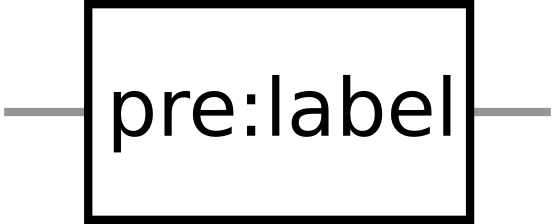
\includegraphics[scale = 0.3]{images/unitInformation}
  \caption{The \ER glyph for \glyph{unit of information}.}
  \label{fig:unitInformation}
\end{figure}

\begin{figure}[H]
  \centering
  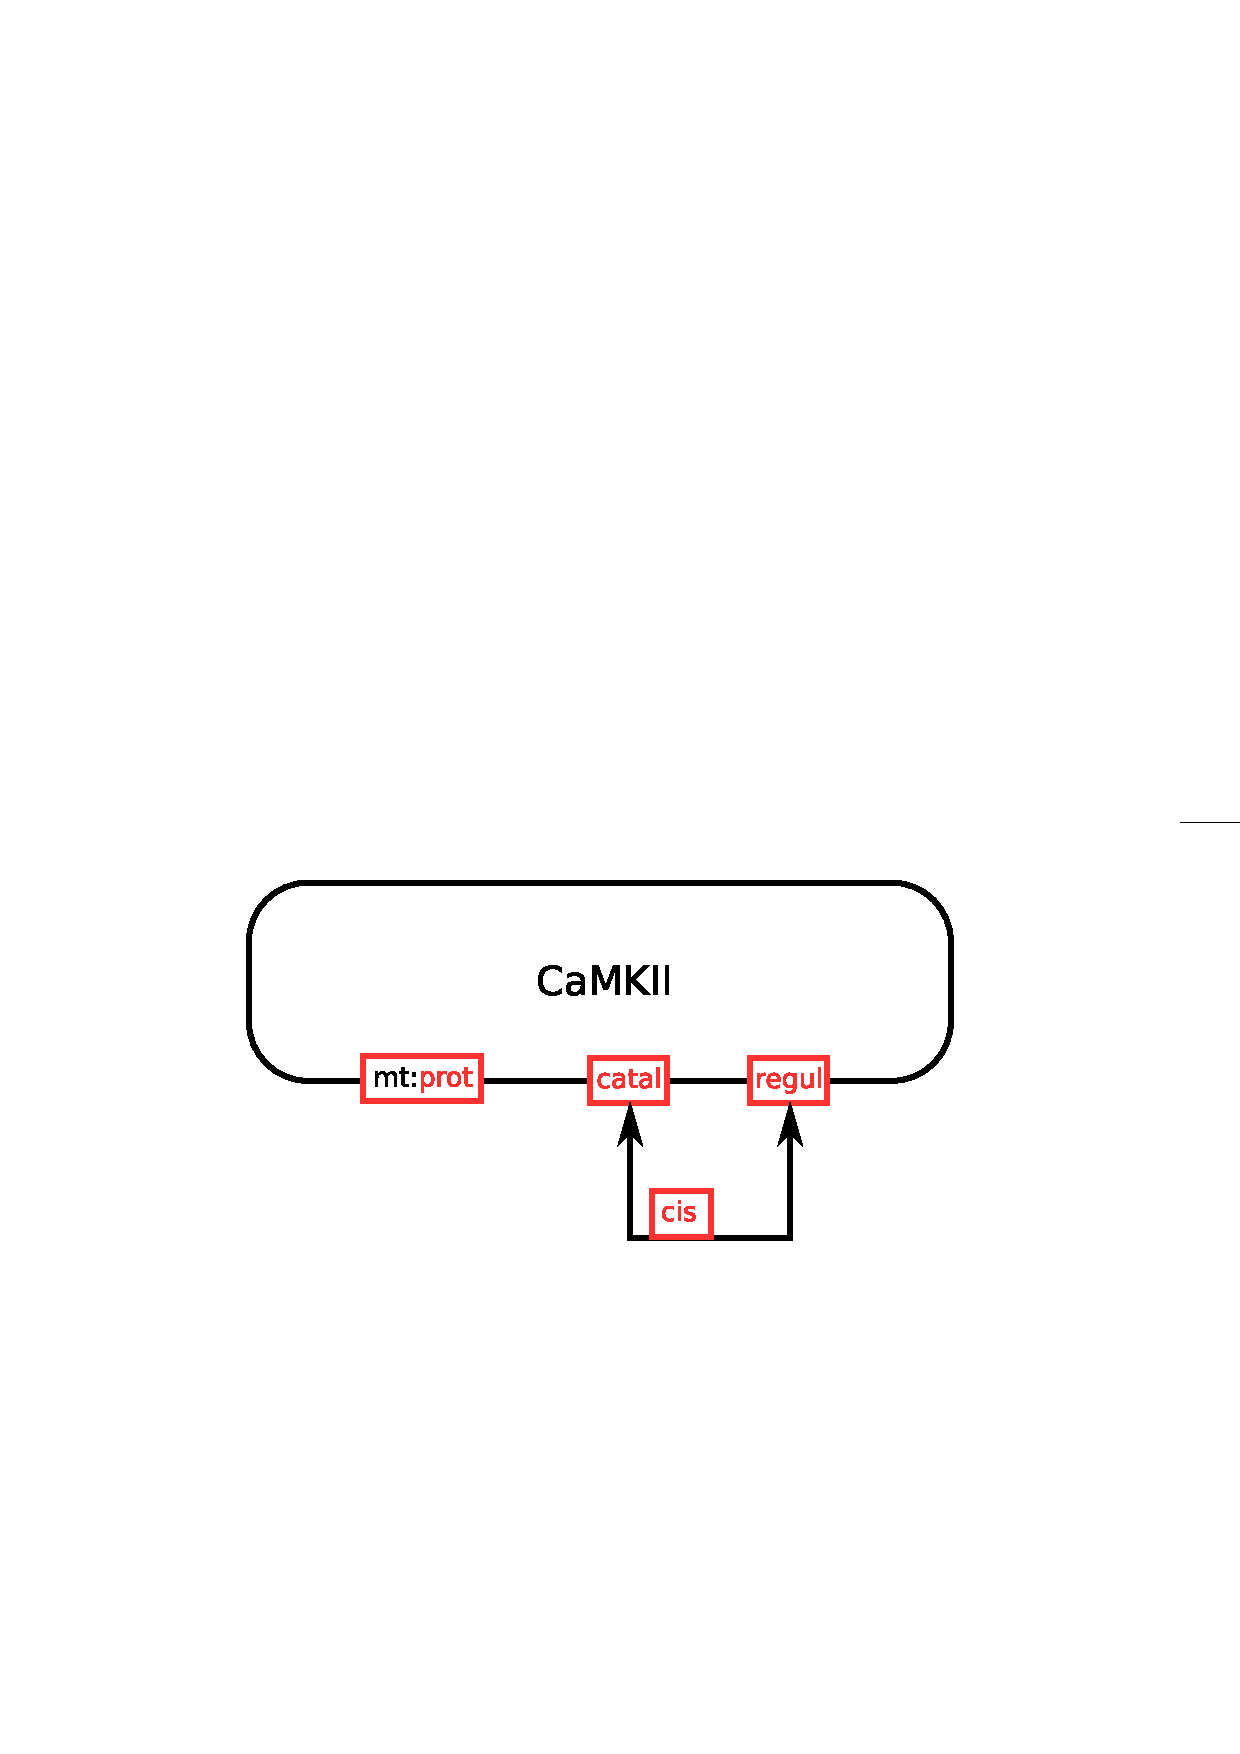
\includegraphics[scale = 0.5]{examples/ex-unitInformation}
  \caption{Using a \glyph{unit of information} to represent the fact that the entity ``CaMKII'' is a protein.}
  \label{fig:ex-unitInformation}
\end{figure}

\normalcolor

%%%%%%%%%%%%%%%%%%%%%%%%%%%%%%%%%%%%%%%%%%%%%%%%%%%%%%%%%%%%%%%%%%%%%%
%%                     State variable
%%%%%%%%%%%%%%%%%%%%%%%%%%%%%%%%%%%%%%%%%%%%%%%%%%%%%%%%%%%%%%%%%%%%%%
%\color{blue}

\subsection{Glyph: \glyph{State variable}}
\label{sec:stateVariable}

Many biological entities such as molecules can exist in different \emph{states}, meaning different physical or informational configurations.  These states can arise for a variety of reasons.  For example, macromolecules can be subject to post-synthesis modifications, wherein residues of the macromolecules (amino acids, nucleosides, or glucid residues) are modified through covalent linkage to other chemicals.  Other examples of states are alternative conformations as in the closed/open/desensitized conformations of a transmembrane channel, and the active/inactive forms of an enzyme.

SBGN provides a means of associating one or more \glyph{state variables} with an entity; each such variable can be used to represent a dimension along which the state of the overall entity can vary.  When an entity can exist in different states, the state of the instance of the entity % (\ie the SBGN object) 
can be described by the current values of all its \glyph{state variables}, and the values of the \glyph{state variables} of all its possible components, recursively.

In \SBGNERLone, \glyph{state variables} are also used to describe the localisation in compartments (a transport is therefore described as a state variable assignment, see \sect{assignment}).

\begin{glyphDescription}

\glyphSboTerm Not applicable.

\glyphContainer A \glyph{state variable} is represented by a ''stadium'' container, that is two semicircles of same radius joined by parallel segments, as shown in \fig{state-var}.  The parallel segment axis should be tangent to the border of the glyph of the \glyph{entity} being modified by the \glyph{state variable}. The center of the bounding box of a \glyph{state variable} should be located on the mid-line of the border of the \glyph{entity}.

\glyphLabel A \glyph{state variable} is identified by a label placed in an unbordered box containing a string of characters.  The characters can be distributed on several lines to improve readability, although this is not mandatory.  The label box must be attached to the center of the container.  The label may spill outside of the container.

\glyphAux A \glyph{state variable} does not carry any auxiliary items.  

\end{glyphDescription}

\begin{figure}[H]
  \centering
  \includegraphics[scale = 0.3]{images/stateVariable}
  \caption{The \ER glyph for \glyph{state variable}. From left to right, horizontal \glyph{state variable}, vertical \glyph{state variable}, \glyph{location}, \glyph{existence}.}
  \label{fig:state-var}
\end{figure}

Two state variables are predefined. The variable \glyph{existence} is used to represent the creation or destruction of entities, as seen on \fig{ex-existence}\label{sec:existence}. \glyph{Existence} can take two values, true (T) or false (F). The variable is represented by a circle vertically divided in two. One hemicircle is black, and the other white. 

\begin{figure}[H]
  \centering
  \includegraphics[scale = 0.5]{examples/ex-existence}
  \caption{Using the \glyph{state variable} \glyph{existence} to represent the appearance of calcium following a depolarisation.}
  \label{fig:ex-existence}
\end{figure}

The variable \glyph{location} is used to represent the physical location of an entity, as seen on \fig{ex-location}\label{sec:location}. \glyph{Location} can take any value, but there can be only one \glyph{location} per instance of an entity. The variable is represented by a circle containing two perpendicular segments, an abstract version of the usual slanted pin.

\begin{figure}[H]
  \centering
  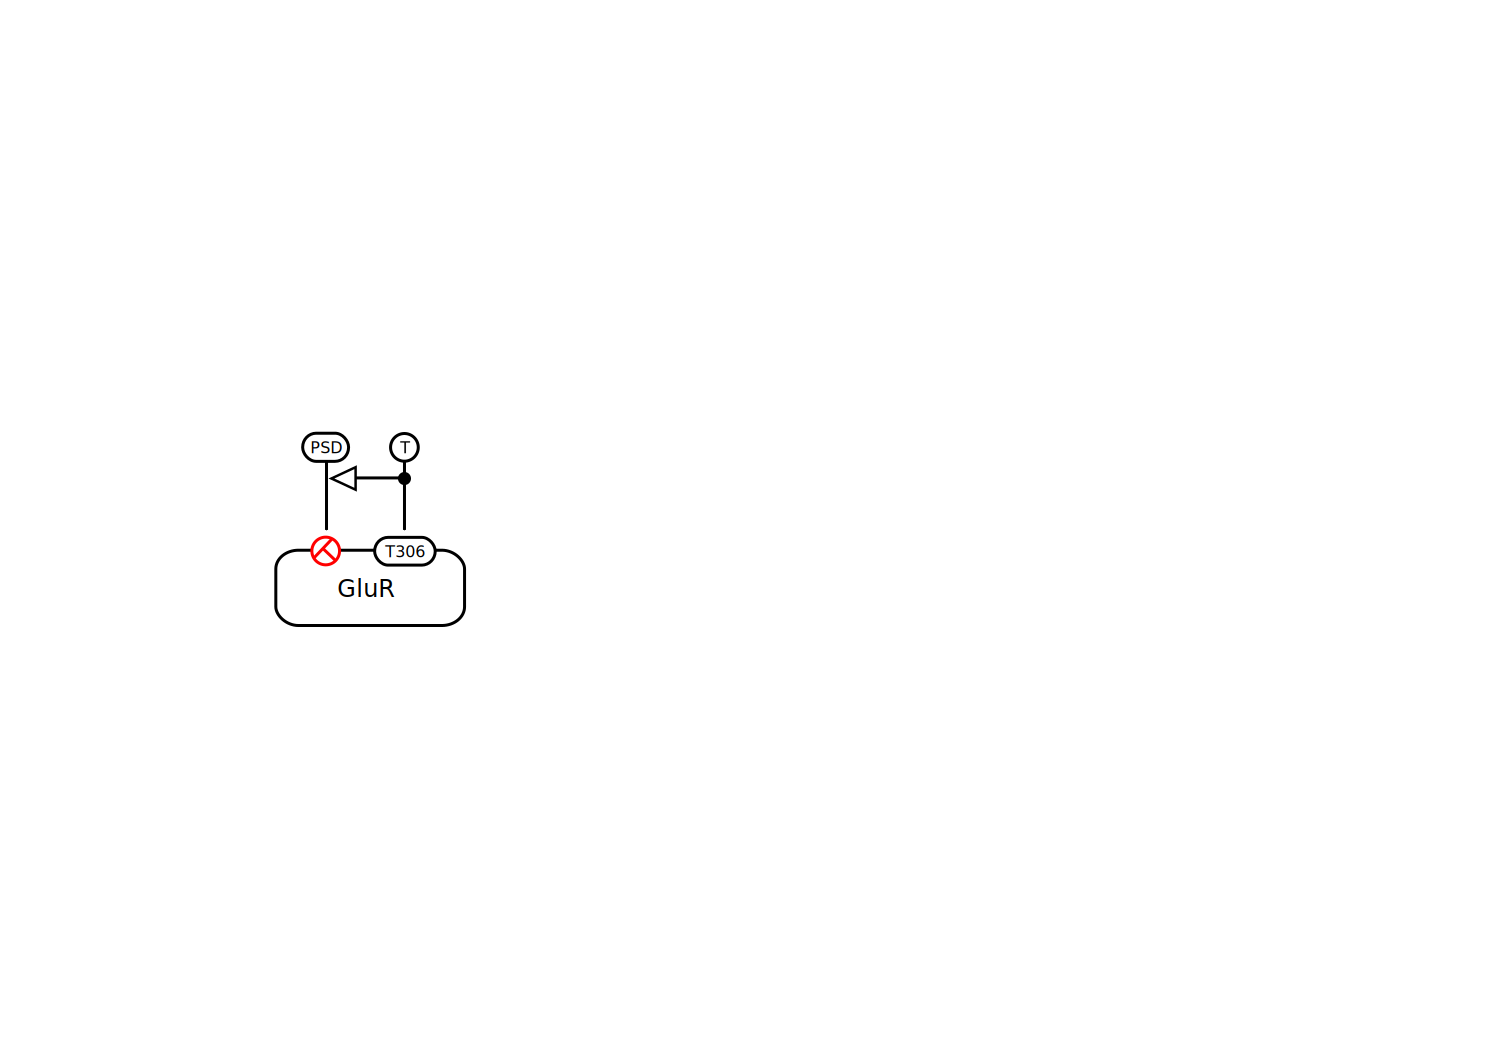
\includegraphics[scale = 0.5]{examples/ex-location-2}
  \caption{Using the \glyph{state variable} \glyph{location} to represent the fact that phosphorylation of glutamate receptors stimulate their incorporation in the post-synaptic density.}
  \label{fig:ex-location}
\end{figure}

%\normalcolor

% The following is for [X]Emacs users.  Please leave in place.
% Local Variables:
% TeX-master: "../sbgn_ER-level1"
% End:


%%%%%%%%%%%%%%%%%%%%%%%%%%%%%%%%%%%%%%%%%%%%%%%%%%%%%%%%%%%%%%%%%%%%%%
%%                     Variable value
%%%%%%%%%%%%%%%%%%%%%%%%%%%%%%%%%%%%%%%%%%%%%%%%%%%%%%%%%%%%%%%%%%%%%%
%\color{blue}

\subsection{Glyph: \glyph{Variable value}}
\label{sec:variableValue}

\begin{glyphDescription}
 
\glyphSboTerm Not applicable.
 
\glyphContainer A \glyph{variable value} is represented by a ''stadium'' container, that is two hemicercles of same radius joined by parallel segments, as shown in \fig{var-value}. 
 
\glyphLabel A \glyph{variable value} is identified by a label placed in an unbordered box containing a string of characters.  The characters can be distributed on several lines to improve readability, although this is not mandatory.  The label box must be attached to the center of the container.  The label may spill outside of the container.

\glyphAux A \glyph{state variable} does not carry any auxiliary items.  
 
\end{glyphDescription}
 
\begin{figure}[H]
   \centering
   \includegraphics[scale = 0.3]{images/variableValue}
   \caption{The \ER glyph for \glyph{state variable}. From left to right, horizontal state variable, vertical state variable, \glyph{Location}, \glyph{existence}.}
   \label{fig:var-value}
\end{figure}

A \glyph{variable value} is linked to a \glyph{state variable} (see \sect{stateVariable}) through \glyph{assignment} (see \sect{assignment}). 

A \glyph{state variable} does not necessarily have to be Boolean-valued.  For example, an ion channel can possess several conductance states; a receptor can be inactive, active and desensitized; and so on.  As another example, a \glyph{state variable} ``ubiquitin'' could also carry numerical values corresponding to the number of ubiquitin molecules present in the tail.

\begin{figure}[H]
  \centering
  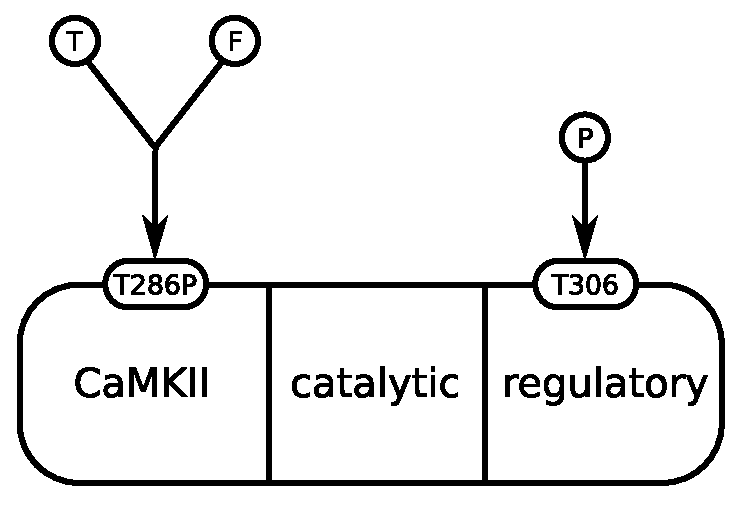
\includegraphics[scale = 0.5]{examples/ex-stateVariable}
  \caption{Two examples of \glyph{state variables} used to represent phophorylation of a threonine residue. While only the value ``phosphorylated'' is assigned to T306, the variable T286P can take the values true or false, which allow for representing dephosphorylation as well as phosphorylation.}
  \label{fig:ex-state-Variable}
\end{figure}

Two state variables are predefined. The variable \glyph{existence} is used to represent the creation or destruction of entities, as seen on \fig{ex-existence}\label{sec:existence}. \glyph{Existence} can take two values, true (T) or false (F). The variable is represented by a circle vertically divided in two. One hemicircle is black, and the other white. 

\begin{figure}[H]
  \centering
  \includegraphics[scale = 0.5]{examples/ex-existence}
  \caption{Using the \glyph{state variable} \glyph{existence} to represent the appearance of calcium following a depolarisation.}
  \label{fig:ex-existence}
\end{figure}

The variable \glyph{location} is used to represent the physical location of an entity, as seen on \fig{ex-location}\label{sec:location}. \glyph{Location} can take any value, but there can be only one \glyph{location} per entity. The variable is represented by a circle containing two perpendicular segments, an abstract version of the usual slanted pin.

\begin{figure}[H]
  \centering
  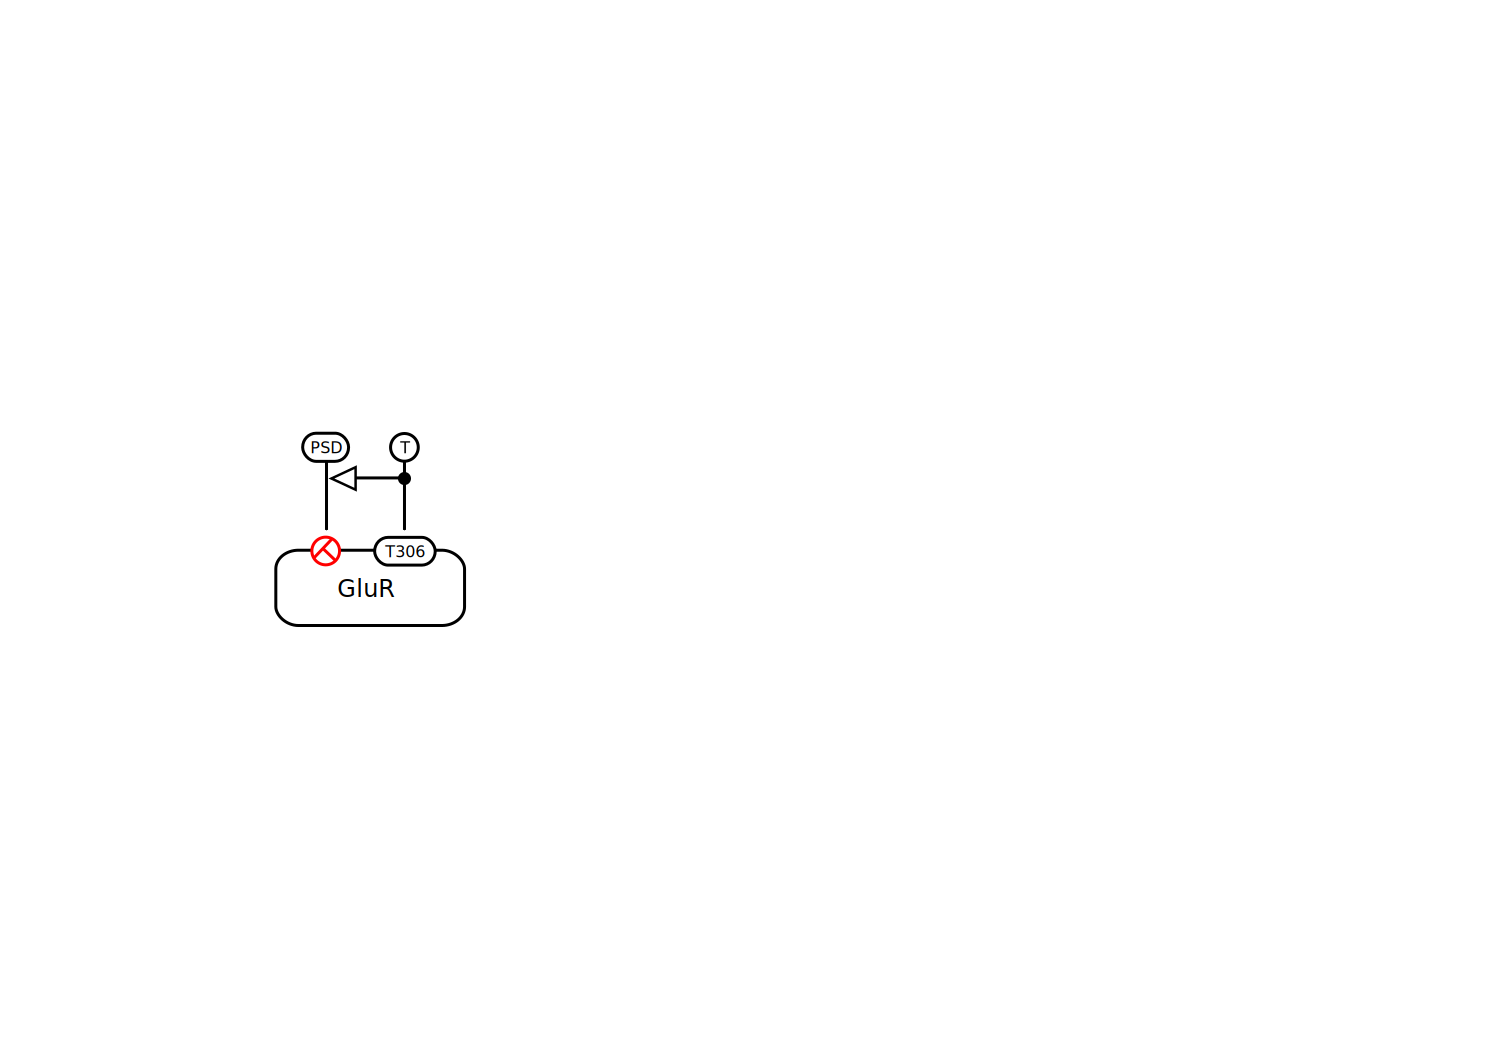
\includegraphics[scale = 0.5]{examples/ex-location-2}
  \caption{Using the \glyph{state variable} \glyph{location} to represent the fact that phosphorylation of glutamate receptors stimulate their incorporation in the post-synaptic density.}
  \label{fig:ex-location}
\end{figure}


% \begin{figure}[H]
%   \centering
%   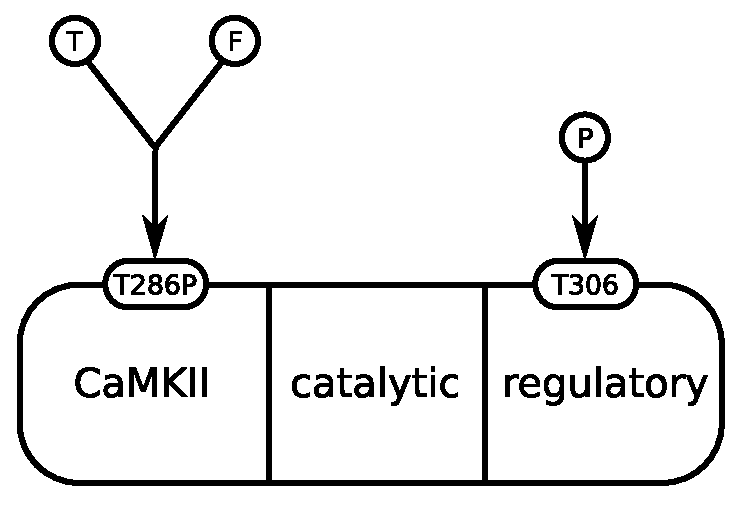
\includegraphics[scale = 0.5]{examples/ex-stateVariable}
%   \caption{Two examples of \glyph{state variables} used to represent phophorylation of a threonine residue. While only the value ``phosphorylated'' is assigned to T306, the variable T286P can take the values true or false, which allow for representing dephosphorylation as well as phosphorylation.}
%   \label{fig:ex-state-Variable}
% \end{figure}
% 
% Two state variables are predefined. The variable \glyph{existence} is used to represent the creation or destruction of entities, as seen on \fig{ex-existence}\label{sec:existence}. \glyph{Existence} can take two values, true (T) or false (F). The variable is represented by a circle vertically divided in two. One hemicircle is black, and the other white. 
% 
% \begin{figure}[H]
%   \centering
%   \includegraphics[scale = 0.5]{examples/ex-existence}
%   \caption{Using the \glyph{state variable} \glyph{existence} to represent the appearance of calcium following a depolarisation.}
%   \label{fig:ex-existence}
% \end{figure}
% 
% The variable \glyph{location} is used to represent the physical location of an entity, as seen on \fig{ex-location}\label{sec:location}. \glyph{Location} can take any value, but there can be only one \glyph{location} per entity. The variable is represented by a circle containing two perpendicular segments, an abstract version of the usual slanted pin.
% 
% \begin{figure}[H]
%   \centering
%   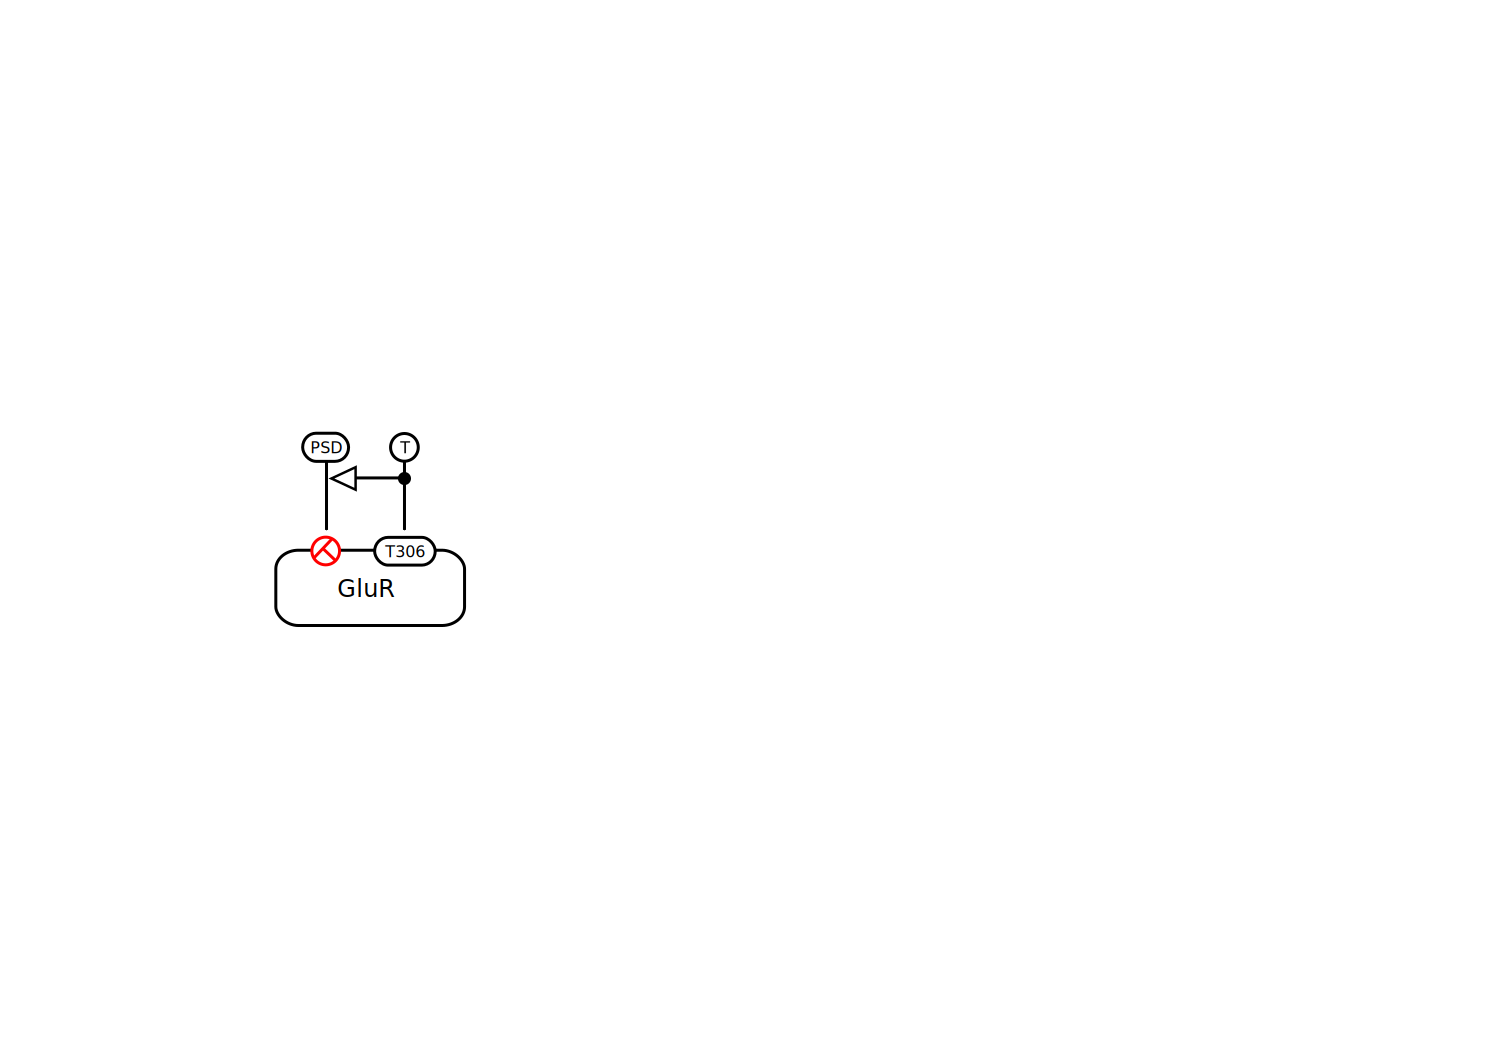
\includegraphics[scale = 0.5]{examples/ex-location-2}
%   \caption{Using the \glyph{state variable} \glyph{location} to represent the fact that phosphorylation of glutamate receptors stimulate their incorporation in the post-synaptic density.}
%   \label{fig:ex-location}
% \end{figure}

%\normalcolor

% The following is for [X]Emacs users.  Please leave in place.
% Local Variables:
% TeX-master: "../sbgn_ER-level1"
% End:


% %%%%%%%%%%%%%%%%%%%%%%%%%%%%%%%%%%%%%%%%%%%%%%%%%%%%%%%%%%%%%%%%%%%%%%
%%                     Domain
%%%%%%%%%%%%%%%%%%%%%%%%%%%%%%%%%%%%%%%%%%%%%%%%%%%%%%%%%%%%%%%%%%%%%%

\subsection{\glyph{Entity} nesting }
\label{sec:domain}

\SBGNERLone Version 2 allows \glyph{entities} to be nested. The relationships between the enclosed \glyph{entity} and the enclosing \glyph{entity} is partship. Note that this relation between \glyph{entities} of different levels does not imply anything about \glyph{entities} of the same level. In the \fig{domain}, A is part of X and B is part of X. However, nothing is said about A and B. A and B could be of different nature (transmembrane domain and transduction domain) or could be overlapping (binding domain and catalytic domain sharing some amino-acids). 

\begin{figure}[H]
  \centering
  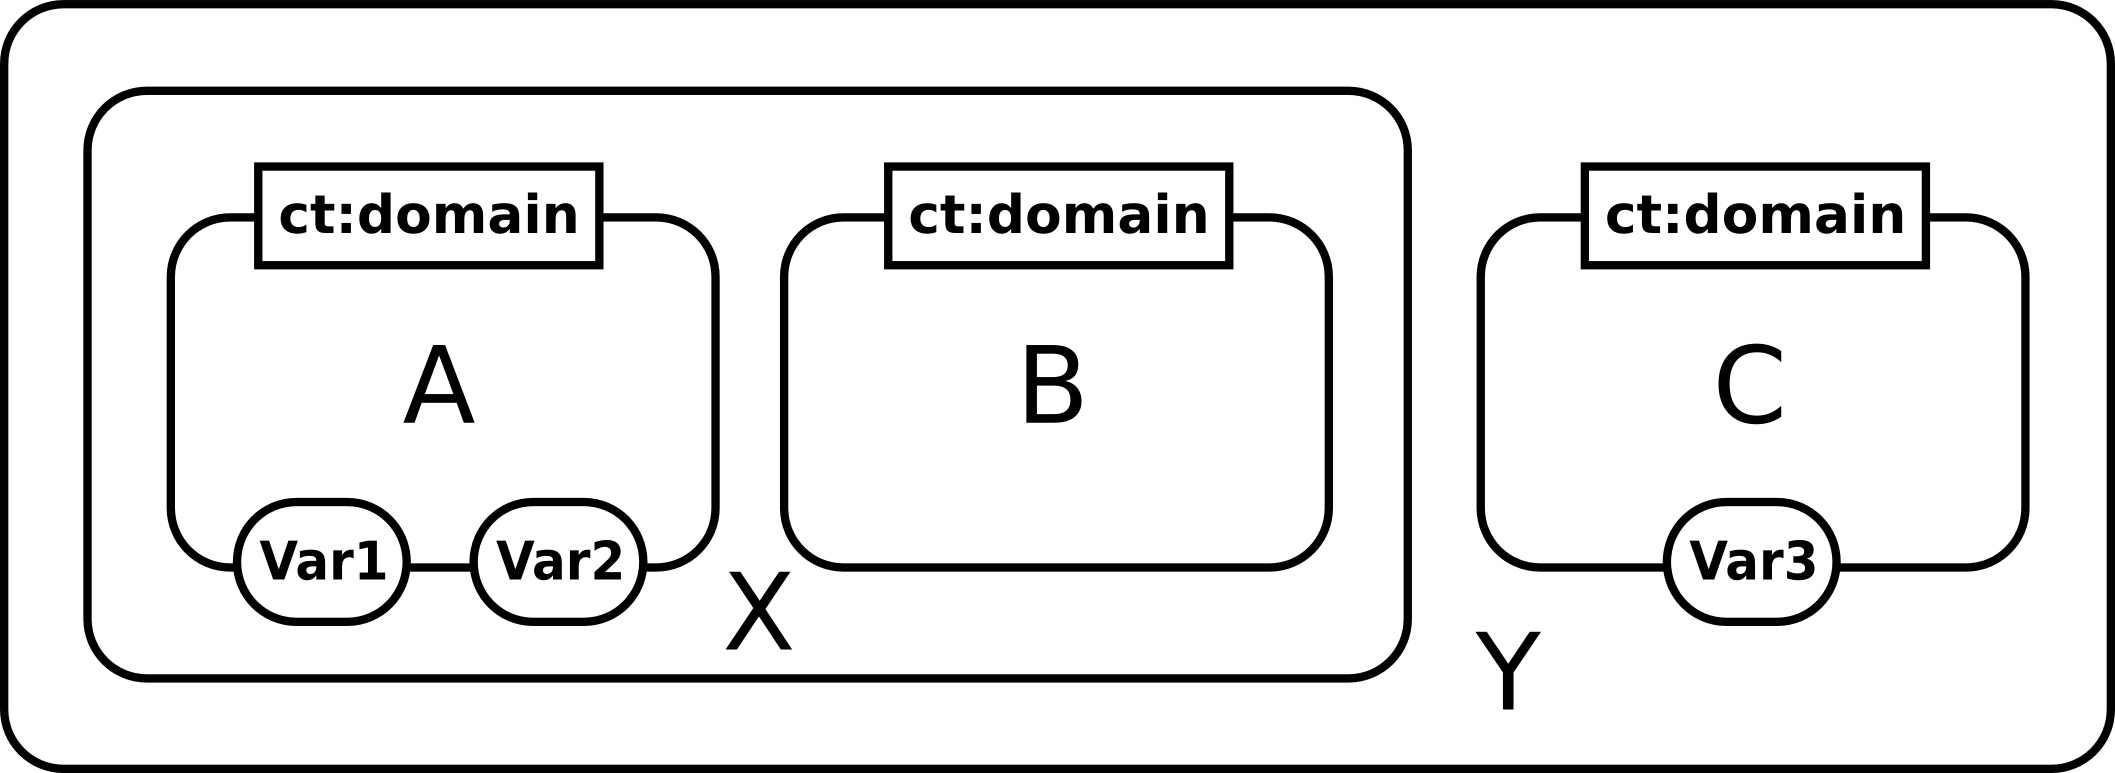
\includegraphics[scale = 0.3]{images/domain}
  \caption{The \ER glyph for \glyph{domain}.}
  \label{fig:domain}
\end{figure}

As any other \glyph{entity}, a nested \glyph{entity} can carry \glyph{state variables} and \glyph{units of information}. The contour of the containing \glyph{entity} must surround the totality of all contained \glyph{entities} including their \glyph{state variables} and \glyph{units of information}. a nested \glyph{entity} can participate to \glyph{interactions}, and generate \glyph{influences}. For more information about the use and interpretation of domains, see \sect{semanticsDomain} 

\begin{figure}[H]
  \centering
  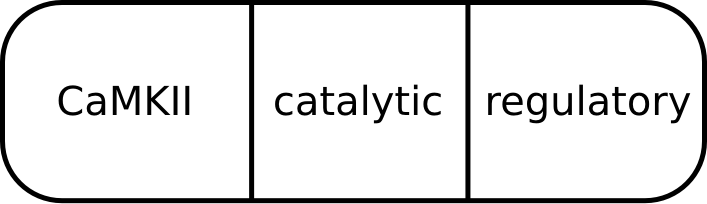
\includegraphics[scale = 0.5]{examples/ex-domain}
  \caption{Illustration of the use of \glyph{domains}. This map contains five \glyph{entities}. Three are top-level, while the \glyph{entities} ``res10-180'' and ``auto-inhibitory'' are domains of the \glyph{entity} ``CaMKII''. The controlled terms carried by the \glyph{units of information} tell us that those \glyph{domains} are a catalytic domain and a binding site respectively.	As far as the relationships with the \glyph{entities} ``calmoduline'' and ``target'' are concerned, the interpretation does not differ from the one we would derive from a map where all the \glyph{entities} would be entirely separated. However the regulation of localisation of ``CaMKII'' to the post-synaptic densite (PSD) by phosphorylation of threonine 286 also causes the localisation of ``res10-180'' and ``auto-inhibitory'', even if none carry the \glyph{state variables} involved.}
  \label{fig:ex-domain}
\end{figure}

\normalcolor               %%%%%% POSTPONED %%%%%%%%
